% Options for packages loaded elsewhere
\PassOptionsToPackage{unicode}{hyperref}
\PassOptionsToPackage{hyphens}{url}
%
\documentclass[
  twocolumn]{article}
\usepackage{amsmath,amssymb}
\usepackage{iftex}
\ifPDFTeX
  \usepackage[T1]{fontenc}
  \usepackage[utf8]{inputenc}
  \usepackage{textcomp} % provide euro and other symbols
\else % if luatex or xetex
  \usepackage{unicode-math} % this also loads fontspec
  \defaultfontfeatures{Scale=MatchLowercase}
  \defaultfontfeatures[\rmfamily]{Ligatures=TeX,Scale=1}
\fi
\usepackage{lmodern}
\ifPDFTeX\else
  % xetex/luatex font selection
  \setmainfont[]{Helvetica}
\fi
% Use upquote if available, for straight quotes in verbatim environments
\IfFileExists{upquote.sty}{\usepackage{upquote}}{}
\IfFileExists{microtype.sty}{% use microtype if available
  \usepackage[]{microtype}
  \UseMicrotypeSet[protrusion]{basicmath} % disable protrusion for tt fonts
}{}
\makeatletter
\@ifundefined{KOMAClassName}{% if non-KOMA class
  \IfFileExists{parskip.sty}{%
    \usepackage{parskip}
  }{% else
    \setlength{\parindent}{0pt}
    \setlength{\parskip}{6pt plus 2pt minus 1pt}}
}{% if KOMA class
  \KOMAoptions{parskip=half}}
\makeatother
\usepackage{xcolor}
\usepackage[margin=1in]{geometry}
\usepackage{graphicx}
\makeatletter
\def\maxwidth{\ifdim\Gin@nat@width>\linewidth\linewidth\else\Gin@nat@width\fi}
\def\maxheight{\ifdim\Gin@nat@height>\textheight\textheight\else\Gin@nat@height\fi}
\makeatother
% Scale images if necessary, so that they will not overflow the page
% margins by default, and it is still possible to overwrite the defaults
% using explicit options in \includegraphics[width, height, ...]{}
\setkeys{Gin}{width=\maxwidth,height=\maxheight,keepaspectratio}
% Set default figure placement to htbp
\makeatletter
\def\fps@figure{htbp}
\makeatother
\setlength{\emergencystretch}{3em} % prevent overfull lines
\providecommand{\tightlist}{%
  \setlength{\itemsep}{0pt}\setlength{\parskip}{0pt}}
\setcounter{secnumdepth}{-\maxdimen} % remove section numbering
\ifLuaTeX
  \usepackage{selnolig}  % disable illegal ligatures
\fi
\IfFileExists{bookmark.sty}{\usepackage{bookmark}}{\usepackage{hyperref}}
\IfFileExists{xurl.sty}{\usepackage{xurl}}{} % add URL line breaks if available
\urlstyle{same}
\hypersetup{
  pdftitle={Curriculum},
  pdfauthor={Joachim Waterschoot},
  hidelinks,
  pdfcreator={LaTeX via pandoc}}

\title{Curriculum}
\author{Joachim Waterschoot\footnote{Department of Developmental,
  Personality and Social Psychology, Ghent University,
  \href{mailto:joachim.waterschoot@ugent.be}{\nolinkurl{joachim.waterschoot@ugent.be}}}}
\date{Latest update - 28 December 2023}

\begin{document}
\maketitle

{
\setcounter{tocdepth}{2}
\tableofcontents
}
\selectfont

\hypertarget{contact-information}{%
\section{\texorpdfstring{Contact information
}{Contact information }}\label{contact-information}}

\begin{center}\rule{0.5\linewidth}{0.5pt}\end{center}

\begin{itemize}
\tightlist
\item
  Email:
  \href{mailto:Joachim.waterschoot@ugent.be}{\nolinkurl{Joachim.waterschoot@ugent.be}}\\
\item
  \href{https://github.com/Watjoa}{Github}\\
\item
  \href{https://www.linkedin.com/in/watjoa}{LinkedIn}\\
\item
  \href{https://www.researchgate.net/profile/Joachim_Waterschoot}{Researchgate}\\
\item
  \href{https://scholar.google.com/citations?user=F-fOgBoAAAAJ\&hl=nl}{Google
  Scholar}
\end{itemize}

TO DO'S:

\begin{itemize}
\tightlist
\item
  Mobility: (a) short-term visit or (b) longer-term mobility planned.
  Goals: to learn new techniques, transfer knowledge, establish/expand
  collaborations.\\
\item
  Teach a course or mentor students: graduate or undergraduate?\\
\item
  Invite and host a collaborator who will give a workshop in your lab.\\
\item
  (Co-)organise a scientific meeting\\
\item
  Develop a database: specify if it is open-access or restricted\\
\item
  Prepare publications in the popular press: name target magazines,
  radio programmes, etc. Mention relevant past experience.\\
\item
  Issue Policy paper: name target organisations, explain what
  relationships will pave the way for conveying your research findings.
\end{itemize}

\hypertarget{education}{%
\section{\texorpdfstring{Education }{Education }}\label{education}}

\begin{center}\rule{0.5\linewidth}{0.5pt}\end{center}

\emph{2017 - 2023}

\textbf{PhD candidate in Developmental and Motivational Psychology}\\
Thesis: The Motivation Barometer during the COVID-19 crisis in Belgium:
The Role of Basic Needs, Risk Perception and Motivation predicting
Behavior and Well-Being. (Supervisors: Prof.~Maarten Vansteenkiste and
Prof.~Bart Soenens)

Ghent University Ghent, Belgium.

\emph{2017 - 2020}

\textbf{MSc in Statistical Data Analysis}\\
Thesis: ``It is not the quantity of motivation that matters'': a
statistical comparison between Cluster analysis and Latent profile
analysis (Supervisors: Prof.~Jan De Neve and Prof.~Wim Beyers)

Ghent University Ghent, Belgium.

\emph{2012 - 2017}

\textbf{MSc in Experimental and Theoretical Psychology}\\
Thesis: Effect of Experimentally Induced Choice on Motivation in Middle
Childhood: The Moderating Role of Teacher and Student Characteristics
(Supervisor: Prof.~Bart Soenens)

Research internship: The Role of Competence-related Attentional Bias and
Resilience in Restoring Thwarted Feelings of Competence at the
Department of Developmental Psychology, Ghent University (Supervisor:
Prof.~Maarten Vansteenkiste)

Ghent University Ghent, Belgium.

\hypertarget{scientific-curriculum}{%
\section{\texorpdfstring{Scientific Curriculum
}{Scientific Curriculum }}\label{scientific-curriculum}}

\begin{center}\rule{0.5\linewidth}{0.5pt}\end{center}

\hypertarget{publications}{%
\subsection{Publications}\label{publications}}


\includegraphics{Vitae_files/figure-latex/unnamed-chunk-2-1.pdf}


\includegraphics{Vitae_files/figure-latex/unnamed-chunk-3-1.pdf}

\hypertarget{by-year}{%
\subsubsection{By year}\label{by-year}}

\hypertarget{section}{%
\paragraph{2024}\label{section}}

\hypertarget{section-1}{%
\paragraph{2023}\label{section-1}}

\begin{enumerate}
\def\labelenumi{\arabic{enumi}.}
\setcounter{enumi}{31}
\tightlist
\item
  Waterschoot, J., Morbée, S., Soenens, B., Van den Bergh, O.,
  Raemdonck, E., Brisbois, M., Schmitz, M., Klein, O., Luminet, O., Van
  Oost, P., Yzerbyt, V., \& Vansteenkiste, M. (2023).
  \textbf{Psychological need fulfillment as a source of resilience: Its
  protective role in concerns and symptoms of anxiety and depression
  during the COVID-19 pandemic.} \emph{Applied psychology. Health and
  well-being, 10}.1111/aphw.12508. Advance online publication.
  \url{https://doi.org/10.1111/aphw.12508}

  \begin{enumerate}
  \def\labelenumii{\arabic{enumii}.}
  \setcounter{enumii}{30}
  \tightlist
  \item
    Waterschoot, J., Morbée, S., Van den Bergh, O., Yzerbyt, V.,
    Raemdonck, E., Brisbois, M., Schmitz, M., Klein, O., Luminet, O.,
    Van Oost, P., \& Vansteenkiste, M. (2023). \textbf{How the
    Stringency of the COVID-19 Restrictions Influences Motivation for
    Adherence and Well-Being: The Critical Role of Proportionality.}
    \emph{International Journal of Health Policy and Management, 12}(1),
    1-13. doi: 10.34172/ijhpm.2023.8021

    \begin{enumerate}
    \def\labelenumiii{\arabic{enumiii}.}
    \setcounter{enumiii}{29}
    \tightlist
    \item
      Waterschoot, J., Van Oost, P., Vansteenkiste, M., Bribois, M.,
      Schmitz, M., Morbée, S., Klein, O., Luminet, O., Van den Bergh,
      O., Raemdonck, E., \& Yzerbyt, V. (2023) \textbf{Who is Motivated
      to Accept a Booster and Annual Dose? A Dimensional and
      Person-Centered Approach.} \emph{Applied Psychology: Health and
      Well-Being, 15}(4), 1293-1318.
      \url{https://doi.org/10.1111/aphw.12437}

      \begin{enumerate}
      \def\labelenumiv{\arabic{enumiv}.}
      \setcounter{enumiv}{28}
      \tightlist
      \item
        Waterschoot, J., Yzerbyt, V., Soenens, B., Van den Bergh, O.,
        Morbée, S., Schmitz, M., Van Oost, P., Luminet, O., Klein, O.,
        \& Vansteenkiste, M. (2023). \textbf{How do vaccination
        intentions change over time? The role of motivational growth.}
        \emph{Health psychology, 42}(2), 113--123.
        \url{https://doi.org/10.1037/hea0001228}

        \begin{enumerate}
        \def\labelenumv{\arabic{enumv}.}
        \tightlist
        \item
          Vansteenkiste, M., Waterschoot, J., Morbée, S., Van Oost, P.,
          Schmitz, M., Klein, O., Luminet, O., Yzerbyt, V., \& Van den
          Bergh, O. (2023). \textbf{Psychologicalscience and its
          societal mission during the SARS-CoV-2 pandemic: The
          Motivation Barometeras an evidence-informed policy instrument
          in Belgium.} \emph{Social Issues and Policy Review,} 1--30.
          \url{https://doi.org/10.1111/sipr.12101}

          \begin{enumerate}
          \def\labelenumvi{\arabic{enumvi}.}
          \tightlist
          \item
            Sypré, S., Waterschoot, J., Soenens, B., Verschueren, K., \&
            Vansteenkiste, M. (2023). \textbf{Do Teachers Use Distinct
            Motivational Styles for Cognitively Gifted Learners? The
            Role of Effectiveness Beliefs, Fixed Mindset, and
            Misconceptions about Giftedness.} \emph{European Journal of
            Psychology of Education,} 1-27.
            \url{https://doi.org/10.1007/s10212-023-00716-2}

            \begin{enumerate}
            \def\labelenumvii{\arabic{enumvii}.}
            \tightlist
            \item
              Morbée, S., Waterschoot, J., De Muynck, G. J., Haerens,
              L., Soenens, B., \& Vansteenkiste, M. (2023).
              \textbf{Identifying profiles of parental (de) motivating
              behaviors in youth sports: A multi-informant approach.}
              \emph{Motivation and Emotion, 47}(6), 990-1006.
              \url{https://doi.org/10.1007/s11031-023-10040-3}

              \begin{enumerate}
              \def\labelenumviii{\arabic{enumviii}.}
              \tightlist
              \item
                van der Kaap‐Deeder, J., Bülow, A., Waterschoot, J.,
                Truyen, I., \& Keijsers, L. (2022). \textbf{A moment of
                autonomy support brightens adolescents' mood: Autonomy
                support, psychological control and adolescent affect in
                everyday life.} \emph{Child Development, early access.}
                \url{http://doi.org/10.1111/cdev.13942}

                \begin{enumerate}
                \def\labelenumix{\arabic{enumix}.}
                \tightlist
                \item
                  Vermote, B., Morbée, S., Soenens, B., Vansteenkiste,
                  M., Waterschoot, J., Beyers, W., \& der Kaap-Deeder,
                  V. (2023). \textbf{How do late adults experience
                  meaning during the COVID-19 lockdown? The role of
                  intrinsic goals.} \emph{Journal of Happiness,} 1-22.
                  \url{https://doi.org/10.1007/s10902-023-00657-z}

                  \begin{enumerate}
                  \def\labelenumx{\arabic{enumx}.}
                  \tightlist
                  \item
                    Morbée, S., Haerens, L., Soenens, B., Loeys, T., De
                    Clerck, T., Waterschoot, J., \& Vansteenkiste, M.
                    (2023). \textbf{Predictors and Outcomes of Sports
                    Coaches' Athlete-Invested Contingent Self-worth.}
                    \emph{Psychology of Sport and Exercise, 69,}102478.
                    \url{https://doi.org/10.1016/j.psychsport.2023.102478}

                    \begin{enumerate}
                    \def\labelenumxi{\arabic{enumxi}.}
                    \tightlist
                    \item
                      Desimpelaere, E., Soenens, B., Prinzie, P.,
                      Waterschoot, J., Vansteenkiste, M., Morbée, S.,
                      Schrooyen, C., \& De Pauw, S. (2023).
                      \textbf{Parents' Stress, Parental Burnout, and
                      Parenting Behavior during the COVID-19 Pandemic:
                      Comparing Parents of Children with and without
                      Complex Care Needs.} \emph{Journal of Child Family
                      Studies, 32}, 3681--3696.
                      \url{https://doi.org/10.1007/s10826-023-02702-0}
                    \end{enumerate}
                  \end{enumerate}
                \end{enumerate}
              \end{enumerate}
            \end{enumerate}
          \end{enumerate}
        \end{enumerate}
      \end{enumerate}
    \end{enumerate}
  \end{enumerate}
\end{enumerate}

\hypertarget{section-2}{%
\paragraph{2022}\label{section-2}}

\begin{enumerate}
\def\labelenumi{\arabic{enumi}.}
\setcounter{enumi}{20}
\tightlist
\item
  Waterschoot, J., Morbée, S., Vermote, B., Brenning, K., Flamant, N.,
  Vansteenkiste, M., \& Soenens, B. (2022). \textbf{Emotion regulation
  in times of COVID-19: A person-centered approach based on
  self-determination theory.} \emph{Current Psychology, 42},
  20211--20225. \url{https://doi.org/10.1007/s12144-021-02623-5}

  \begin{enumerate}
  \def\labelenumii{\arabic{enumii}.}
  \setcounter{enumii}{19}
  \tightlist
  \item
    Waterschoot, J., Morbée, S., Van den Bergh, O., \& Vansteenkiste, M.
    (2022). \textbf{Merry Christmas and a `Healthy' New Year: Assessing
    people's Expectations regarding Christmas Gathering in Pandemic
    Times.} \emph{European Journal of Health Psychology, 30}(1), 17--28.
    \url{https://doi.org/10.1027/2512-8442/a000114}.

    \begin{enumerate}
    \def\labelenumiii{\arabic{enumiii}.}
    \setcounter{enumiii}{18}
    \tightlist
    \item
      Brenning, K., Waterschoot, J., Dieleman, L., Morbée, S., Vermote,
      B., Soenens, B., Van der Kaap-Deeder, J., van den Bogaard, D., \&
      Vansteenkiste, M. (2022). \textbf{Maladaptive Emotion Regulation
      as a Vulnerability Factor during the COVID-19 Pandemic: A 10-Wave
      Longitudinal Study.} \emph{Stress \& Health, 39}(3), 562-575.
      \url{https://doi.org/10.1002/smi.3204}

      \begin{enumerate}
      \def\labelenumiv{\arabic{enumiv}.}
      \setcounter{enumiv}{17}
      \tightlist
      \item
        Morbée, S., Waterschoot, J., Yzerbyt, V., Klein, O., Luminet,
        O., Schmitz, M., Van den Bergh, O., Van Oost, P., De Craene, S.,
        \& Vansteenkiste, M. (2022). \textbf{Personal and contextual
        determinants of COVID-19 vaccination intention: a vignette
        study.} \emph{Expert review of vaccines, 21}(10), 1475-1485.
        \url{https://doi.org/10.1080/14760584.2022.2105212}

        \begin{enumerate}
        \def\labelenumv{\arabic{enumv}.}
        \tightlist
        \item
          Van de Casteele, M., Waterschoot, J., Anthierens, S., DeSmet,
          A., Galand, B., Goossens, H., Morbée, S., \& Vansteenkiste, M.
          (2022). \textbf{Saliva testing among teachers during the
          COVID-19 pandemic: Effects on health concerns, well-being, and
          precautionary behavior.} \emph{Social Science \& Medicine,
          311,} 115295. \url{doi:10.1016/j.socscimed.2022.115295}

          \begin{enumerate}
          \def\labelenumvi{\arabic{enumvi}.}
          \tightlist
          \item
            Vansteenkiste, M, Soenens, B., \& Waterschoot, J., (2022).
            \textbf{Catalyzing Intrinsic and Internalized Motivation:
            The Role of Basic Psychological Needs and Their Support}, in
            O'Donnell, A., Barnes, N., C., \& Reeve, J. (eds), \emph{The
            Oxford Handbook of Educational Psychology} (online edn,
            Oxford Academic, 5 Apr.~2018).
            \url{https://doi.org/10.1093/oxfordhb/9780199841332.013.41}

            \begin{enumerate}
            \def\labelenumvii{\arabic{enumvii}.}
            \tightlist
            \item
              Morbée, S., Vansteenkiste, M., Waterschoot, J., Klein, O.,
              Luminet, O., Schmitz, M., Van den Bergh, O., Van Oost, P.,
              \& Yzerbyt, V. (2022). \textbf{The Role of Communication
              Style and External Motivators in Predicting Vaccination
              Experiences and Intentions: An Experimental Vignette
              Study.} \emph{Health communication}, 1-10.
              \url{https://doi.org/10.1080/10410236.2022.2125012}

              \begin{enumerate}
              \def\labelenumviii{\arabic{enumviii}.}
              \tightlist
              \item
                Morbée, S., Beeckman, M., Loeys, T., Waterschoot, J.,
                Cardon, G., Haerens, L., \& Vansteenkiste, M. \textbf{A
                Brief Report on the Reciprocal Associations between
                Physical Activity and Mental Well-being during the First
                9 Weeks of the COVID-19 Lockdown in Belgium.}
                \emph{Mental Health and Physical Activity, 24}, 100500.
                \url{https://doi.org/10.1016/j.mhpa.2022.100500}

                \begin{enumerate}
                \def\labelenumix{\arabic{enumix}.}
                \tightlist
                \item
                  Wauters, A., Vervoort, T., Dhondt, K., Soenens, B.,
                  Vansteenkiste, M., Morbée, S., Waterschoot, J.,
                  Haerynck, F., Vandekerckhove, K., Verhelst, H., Van
                  Aken, S., Raes, A., Schelstraete, P., Vande Walle, J.,
                  \& Van Hoecke, E. (2022). \textbf{Mental health
                  outcomes among parents of children with a chronic
                  disease during the COVID-19 pandemic: The role of
                  parental burn-out.} \emph{Journal of Pediatric
                  Psychology, 47}(4), 420-431.
                  \url{https://doi.org/10.1093/jpepsy/jsab129}

                  \begin{enumerate}
                  \def\labelenumx{\arabic{enumx}.}
                  \tightlist
                  \item
                    Schmitz, M., Luminet, O., Klein, O., Morbée, S., Van
                    den Bergh, O., Van Oost, P., Waterschoot, J.,
                    Yzerbyt, V., \& Vansteenkiste, M. (2022).
                    \textbf{Predicting vaccine uptake during COVID-19
                    crisis: A motivational approach.} \emph{Vaccine,
                    40}(2), 288-297.
                    \url{https://doi.org/10.1016/j.vaccine.2021.11.068}
                    (2022).

                    \begin{enumerate}
                    \def\labelenumxi{\arabic{enumxi}.}
                    \tightlist
                    \item
                      Van Oost, P., Yzerbyt, V., Schmitz, M.,
                      Vansteenkiste, M., Luminet, O., Morbée, S., Van
                      den Bergh, O., Waterschoot, J., \& Klein, O.
                      (2022). \textbf{The relation between conspiracism,
                      government trust, and COVID-19 vaccination
                      intentions: The key role of motivation.}
                      \emph{Social Science \& Medicine, 301}, 114926.
                      \url{https://doi.org/10.1016/j.socscimed.2022.114926}

                      \begin{enumerate}
                      \def\labelenumxii{\arabic{enumxii}.}
                      \tightlist
                      \item
                        Legate, N., Ngyuen, T. V., Weinstein, N.,
                        Moller, A., Legault, L., Vally, Z., \ldots{} \&
                        Ogbonnaya, C. E. (2022). \textbf{A global
                        experiment on motivating social distancing
                        during the COVID-19 pandemic.} \emph{Proceedings
                        of the National Academy of Sciences, 119}(22).
                        \url{https://doi.org/10.1073/pnas.2111091119}
                      \end{enumerate}
                    \end{enumerate}
                  \end{enumerate}
                \end{enumerate}
              \end{enumerate}
            \end{enumerate}
          \end{enumerate}
        \end{enumerate}
      \end{enumerate}
    \end{enumerate}
  \end{enumerate}
\end{enumerate}

\hypertarget{section-3}{%
\paragraph{2021}\label{section-3}}

\begin{enumerate}
\def\labelenumi{\arabic{enumi}.}
\setcounter{enumi}{8}
\tightlist
\item
  Waterschoot, J., Van der Kaap-Deeder, J., Morbée, S., Soenens, B., \&
  Vansteenkiste, M. (2021). \textbf{``How to unlock myself from
  boredom?'' The role of mindfulness and a dual awareness-and
  action-oriented pathway during the COVID-19 lockdown.}
  \emph{Personality and Individual Differences, 175,} 110729.
  \url{https://doi.org/10.1016/j.paid.2021.110729}

  \begin{enumerate}
  \def\labelenumii{\arabic{enumii}.}
  \setcounter{enumii}{7}
  \tightlist
  \item
    Vermote, B., Waterschoot, J., Morbée, S., Van der Kaap-Deeder, J.,
    Schrooyen, C., Soenens, B., Ryan, R., \& Vansteenkiste, M. (2022).
    \textbf{Do Psychological Needs Play a Role in Times of Uncertainty?
    Associations with Well-Being During the COVID-19 Crisis.}
    \emph{Journal of happiness studies, 23}(1), 257--283.
    \url{https://doi.org/10.1007/s10902-021-00398-x}

    \begin{enumerate}
    \def\labelenumiii{\arabic{enumiii}.}
    \setcounter{enumiii}{6}
    \tightlist
    \item
      Morbée, S., Haerens, L., Waterschoot, J., \& Vansteenkiste, M.
      (2021). \textbf{Which cyclists manage to cope with the corona
      crisis in a resilient way? The role of motivational profiles.}
      \emph{International Journal of Sport and Exercise Psychology,}
      1-19. \url{https://doi.org/10.1080/1612197X.2021.1940241}

      \begin{enumerate}
      \def\labelenumiv{\arabic{enumiv}.}
      \setcounter{enumiv}{5}
      \tightlist
      \item
        Morbée, S., Vermote, B., Waterschoot, J., Dieleman, L., Soenens,
        B., Van den Bergh, O., Ryan, R. M., Vanhalst, J., De Muynck,
        G.-J., \& Vansteenkiste, M. (2021). \textbf{Adherence to
        COVID-19 measures: The critical role of autonomous motivation on
        a short- and long-term basis.} \emph{Motivation Science, 7}(4),
        487--496. \url{https://doi.org/10.1037/mot0000250}

        \begin{enumerate}
        \def\labelenumv{\arabic{enumv}.}
        \tightlist
        \item
          Schrooyen, C., Soenens, B., Waterschoot, J., Vermote, B.,
          Morbée, S., Beyers, W., Brenning, K., Dieleman, L., Van der
          Kaap-Deeder, J., \& Vansteenkiste, M. (2021). \textbf{Parental
          identity as a resource for parental adaptation during the
          COVID-19 lockdown.} \emph{Journal of Family Psychology,
          35}(8), 1053-1064. \url{https://doi.org/10.1037/fam0000895}

          \begin{enumerate}
          \def\labelenumvi{\arabic{enumvi}.}
          \tightlist
          \item
            van der Kaap-Deeder, J., Vermote, B., Waterschoot, J.,
            Soenens, B., Morbée, S., \& Vansteenkiste, M.
            (2021).\textbf{The role of ego integrity and despair in
            older adults' well-being during the COVID-19 crisis: the
            mediating role of need-based experiences.} \emph{European
            Journal of Ageing, 19}, 117--129.
            \url{https://doi.org/10.1007/s10433-021-00610-0}
          \end{enumerate}
        \end{enumerate}
      \end{enumerate}
    \end{enumerate}
  \end{enumerate}
\end{enumerate}

\hypertarget{section-4}{%
\paragraph{2020}\label{section-4}}

\begin{enumerate}
\def\labelenumi{\arabic{enumi}.}
\setcounter{enumi}{2}
\tightlist
\item
  Waterschoot, J., van der Kaap-Deeder, J., \& Vansteenkiste, M. (2020).
  \textbf{The role of competence-related attentional bias and resilience
  in restoring thwarted feelings of competence.} \emph{Motivation and
  Emotion, 44}(1), 82-98.
  \url{https://doi.org/10.1007/s11031-019-09776-8}
\end{enumerate}

\hypertarget{section-5}{%
\paragraph{2019}\label{section-5}}

\begin{enumerate}
\def\labelenumi{\arabic{enumi}.}
\setcounter{enumi}{1}
\tightlist
\item
  Waterschoot, J., Vansteenkiste, M., \& Soenens, B. (2019). \textbf{The
  effects of experimentally induced choice on elementary school
  children's intrinsic motivation: The moderating role of indecisiveness
  and teacher--student relatedness.} \emph{Journal of experimental child
  psychology, 188,} 104692.
  \url{https://doi.org/10.1016/j.jecp.2019.104692}

  \begin{enumerate}
  \def\labelenumii{\arabic{enumii}.}
  \tightlist
  \item
    De Muynck, G. J., Soenens, B., Waterschoot, J., Degraeuwe, L.,
    Broek, G. V., \& Vansteenkiste, M. (2019). \textbf{Towards a more
    refined insight in the critical motivating features of choice: An
    experimental study among recreational rope skippers.}
    \emph{Psychology of Sport and Exercise, 45}, 101561.
    \url{https://doi.org/10.1016/j.psychsport.2019.101561}
  \end{enumerate}
\end{enumerate}

\hypertarget{by-theme}{%
\subsubsection{By theme}\label{by-theme}}

covid19

\begin{enumerate}
\def\labelenumi{\arabic{enumi}.}
\setcounter{enumi}{31}
\tightlist
\item
  Waterschoot, J., Morbée, S., Soenens, B., Van den Bergh, O.,
  Raemdonck, E., Brisbois, M., Schmitz, M., Klein, O., Luminet, O., Van
  Oost, P., Yzerbyt, V., \& Vansteenkiste, M. (2023).
  \textbf{Psychological need fulfillment as a source of resilience: Its
  protective role in concerns and symptoms of anxiety and depression
  during the COVID-19 pandemic.} \emph{Applied psychology. Health and
  well-being, 10}.1111/aphw.12508. Advance online publication.
  \url{https://doi.org/10.1111/aphw.12508}

  covid19

  \begin{enumerate}
  \def\labelenumii{\arabic{enumii}.}
  \setcounter{enumii}{30}
  \tightlist
  \item
    Waterschoot, J., Morbée, S., Van den Bergh, O., Yzerbyt, V.,
    Raemdonck, E., Brisbois, M., Schmitz, M., Klein, O., Luminet, O.,
    Van Oost, P., \& Vansteenkiste, M. (2023). \textbf{How the
    Stringency of the COVID-19 Restrictions Influences Motivation for
    Adherence and Well-Being: The Critical Role of Proportionality.}
    \emph{International Journal of Health Policy and Management, 12}(1),
    1-13. doi: 10.34172/ijhpm.2023.8021

    covid19

    \begin{enumerate}
    \def\labelenumiii{\arabic{enumiii}.}
    \setcounter{enumiii}{29}
    \tightlist
    \item
      Waterschoot, J., Van Oost, P., Vansteenkiste, M., Bribois, M.,
      Schmitz, M., Morbée, S., Klein, O., Luminet, O., Van den Bergh,
      O., Raemdonck, E., \& Yzerbyt, V. (2023) \textbf{Who is Motivated
      to Accept a Booster and Annual Dose? A Dimensional and
      Person-Centered Approach.} \emph{Applied Psychology: Health and
      Well-Being, 15}(4), 1293-1318.
      \url{https://doi.org/10.1111/aphw.12437}

      covid19

      \begin{enumerate}
      \def\labelenumiv{\arabic{enumiv}.}
      \setcounter{enumiv}{28}
      \tightlist
      \item
        Waterschoot, J., Yzerbyt, V., Soenens, B., Van den Bergh, O.,
        Morbée, S., Schmitz, M., Van Oost, P., Luminet, O., Klein, O.,
        \& Vansteenkiste, M. (2023). \textbf{How do vaccination
        intentions change over time? The role of motivational growth.}
        \emph{Health psychology, 42}(2), 113--123.
        \url{https://doi.org/10.1037/hea0001228}

        covid19

        \begin{enumerate}
        \def\labelenumv{\arabic{enumv}.}
        \tightlist
        \item
          Vansteenkiste, M., Waterschoot, J., Morbée, S., Van Oost, P.,
          Schmitz, M., Klein, O., Luminet, O., Yzerbyt, V., \& Van den
          Bergh, O. (2023). \textbf{Psychologicalscience and its
          societal mission during the SARS-CoV-2 pandemic: The
          Motivation Barometeras an evidence-informed policy instrument
          in Belgium.} \emph{Social Issues and Policy Review,} 1--30.
          \url{https://doi.org/10.1111/sipr.12101}

          covid19

          \begin{enumerate}
          \def\labelenumvi{\arabic{enumvi}.}
          \tightlist
          \item
            Morbée, S., Waterschoot, J., De Muynck, G. J., Haerens, L.,
            Soenens, B., \& Vansteenkiste, M. (2023).
            \textbf{Identifying profiles of parental (de) motivating
            behaviors in youth sports: A multi-informant approach.}
            \emph{Motivation and Emotion, 47}(6), 990-1006.
            \url{https://doi.org/10.1007/s11031-023-10040-3}

            covid19

            \begin{enumerate}
            \def\labelenumvii{\arabic{enumvii}.}
            \tightlist
            \item
              Vermote, B., Morbée, S., Soenens, B., Vansteenkiste, M.,
              Waterschoot, J., Beyers, W., \& der Kaap-Deeder, V.
              (2023). \textbf{How do late adults experience meaning
              during the COVID-19 lockdown? The role of intrinsic
              goals.} \emph{Journal of Happiness,} 1-22.
              \url{https://doi.org/10.1007/s10902-023-00657-z}

              covid19

              \begin{enumerate}
              \def\labelenumviii{\arabic{enumviii}.}
              \tightlist
              \item
                Waterschoot, J., Morbée, S., Vermote, B., Brenning, K.,
                Flamant, N., Vansteenkiste, M., \& Soenens, B. (2022).
                \textbf{Emotion regulation in times of COVID-19: A
                person-centered approach based on self-determination
                theory.} \emph{Current Psychology, 42}, 20211--20225.
                \url{https://doi.org/10.1007/s12144-021-02623-5}

                covid19

                \begin{enumerate}
                \def\labelenumix{\arabic{enumix}.}
                \tightlist
                \item
                  Waterschoot, J., Morbée, S., Van den Bergh, O., \&
                  Vansteenkiste, M. (2022). \textbf{Merry Christmas and
                  a `Healthy' New Year: Assessing people's Expectations
                  regarding Christmas Gathering in Pandemic Times.}
                  \emph{European Journal of Health Psychology, 30}(1),
                  17--28.
                  \url{https://doi.org/10.1027/2512-8442/a000114}.

                  covid19

                  \begin{enumerate}
                  \def\labelenumx{\arabic{enumx}.}
                  \tightlist
                  \item
                    Brenning, K., Waterschoot, J., Dieleman, L., Morbée,
                    S., Vermote, B., Soenens, B., Van der Kaap-Deeder,
                    J., van den Bogaard, D., \& Vansteenkiste, M.
                    (2022). \textbf{Maladaptive Emotion Regulation as a
                    Vulnerability Factor during the COVID-19 Pandemic: A
                    10-Wave Longitudinal Study.} \emph{Stress \& Health,
                    39}(3), 562-575.
                    \url{https://doi.org/10.1002/smi.3204}

                    covid19

                    \begin{enumerate}
                    \def\labelenumxi{\arabic{enumxi}.}
                    \tightlist
                    \item
                      Morbée, S., Waterschoot, J., Yzerbyt, V., Klein,
                      O., Luminet, O., Schmitz, M., Van den Bergh, O.,
                      Van Oost, P., De Craene, S., \& Vansteenkiste, M.
                      (2022). \textbf{Personal and contextual
                      determinants of COVID-19 vaccination intention: a
                      vignette study.} \emph{Expert review of vaccines,
                      21}(10), 1475-1485.
                      \url{https://doi.org/10.1080/14760584.2022.2105212}

                      covid19

                      \begin{enumerate}
                      \def\labelenumxii{\arabic{enumxii}.}
                      \tightlist
                      \item
                        Van de Casteele, M., Waterschoot, J.,
                        Anthierens, S., DeSmet, A., Galand, B.,
                        Goossens, H., Morbée, S., \& Vansteenkiste, M.
                        (2022). \textbf{Saliva testing among teachers
                        during the COVID-19 pandemic: Effects on health
                        concerns, well-being, and precautionary
                        behavior.} \emph{Social Science \& Medicine,
                        311,} 115295.
                        \url{doi:10.1016/j.socscimed.2022.115295}

                        covid19

                        \begin{enumerate}
                        \def\labelenumxiii{\arabic{enumxiii}.}
                        \tightlist
                        \item
                          Morbée, S., Vansteenkiste, M., Waterschoot,
                          J., Klein, O., Luminet, O., Schmitz, M., Van
                          den Bergh, O., Van Oost, P., \& Yzerbyt, V.
                          (2022). \textbf{The Role of Communication
                          Style and External Motivators in Predicting
                          Vaccination Experiences and Intentions: An
                          Experimental Vignette Study.} \emph{Health
                          communication}, 1-10.
                          \url{https://doi.org/10.1080/10410236.2022.2125012}

                          covid19

                          \begin{enumerate}
                          \def\labelenumxiv{\arabic{enumxiv}.}
                          \tightlist
                          \item
                            Morbée, S., Beeckman, M., Loeys, T.,
                            Waterschoot, J., Cardon, G., Haerens, L., \&
                            Vansteenkiste, M. \textbf{A Brief Report on
                            the Reciprocal Associations between Physical
                            Activity and Mental Well-being during the
                            First 9 Weeks of the COVID-19 Lockdown in
                            Belgium.} \emph{Mental Health and Physical
                            Activity, 24}, 100500.
                            \url{https://doi.org/10.1016/j.mhpa.2022.100500}

                            covid19

                            \begin{enumerate}
                            \def\labelenumxv{\arabic{enumxv}.}
                            \tightlist
                            \item
                              Wauters, A., Vervoort, T., Dhondt, K.,
                              Soenens, B., Vansteenkiste, M., Morbée,
                              S., Waterschoot, J., Haerynck, F.,
                              Vandekerckhove, K., Verhelst, H., Van
                              Aken, S., Raes, A., Schelstraete, P.,
                              Vande Walle, J., \& Van Hoecke, E. (2022).
                              \textbf{Mental health outcomes among
                              parents of children with a chronic disease
                              during the COVID-19 pandemic: The role of
                              parental burn-out.} \emph{Journal of
                              Pediatric Psychology, 47}(4), 420-431.
                              \url{https://doi.org/10.1093/jpepsy/jsab129}

                              covid19

                              \begin{enumerate}
                              \def\labelenumxvi{\arabic{enumxvi}.}
                              \tightlist
                              \item
                                Schmitz, M., Luminet, O., Klein, O.,
                                Morbée, S., Van den Bergh, O., Van Oost,
                                P., Waterschoot, J., Yzerbyt, V., \&
                                Vansteenkiste, M. (2022).
                                \textbf{Predicting vaccine uptake during
                                COVID-19 crisis: A motivational
                                approach.} \emph{Vaccine, 40}(2),
                                288-297.
                                \url{https://doi.org/10.1016/j.vaccine.2021.11.068}
                                (2022).

                                covid19

                                \begin{enumerate}
                                \def\labelenumxvii{\arabic{enumxvii}.}
                                \tightlist
                                \item
                                  Van Oost, P., Yzerbyt, V., Schmitz,
                                  M., Vansteenkiste, M., Luminet, O.,
                                  Morbée, S., Van den Bergh, O.,
                                  Waterschoot, J., \& Klein, O. (2022).
                                  \textbf{The relation between
                                  conspiracism, government trust, and
                                  COVID-19 vaccination intentions: The
                                  key role of motivation.} \emph{Social
                                  Science \& Medicine, 301}, 114926.
                                  \url{https://doi.org/10.1016/j.socscimed.2022.114926}

                                  covid19

                                  \begin{enumerate}
                                  \def\labelenumxviii{\arabic{enumxviii}.}
                                  \tightlist
                                  \item
                                    Legate, N., Ngyuen, T. V.,
                                    Weinstein, N., Moller, A., Legault,
                                    L., Vally, Z., \ldots{} \&
                                    Ogbonnaya, C. E. (2022). \textbf{A
                                    global experiment on motivating
                                    social distancing during the
                                    COVID-19 pandemic.}
                                    \emph{Proceedings of the National
                                    Academy of Sciences, 119}(22).
                                    \url{https://doi.org/10.1073/pnas.2111091119}

                                    covid19

                                    \begin{enumerate}
                                    \def\labelenumxix{\arabic{enumxix}.}
                                    \tightlist
                                    \item
                                      Waterschoot, J., Van der
                                      Kaap-Deeder, J., Morbée, S.,
                                      Soenens, B., \& Vansteenkiste, M.
                                      (2021). \textbf{``How to unlock
                                      myself from boredom?'' The role of
                                      mindfulness and a dual
                                      awareness-and action-oriented
                                      pathway during the COVID-19
                                      lockdown.} \emph{Personality and
                                      Individual Differences, 175,}
                                      110729.
                                      \url{https://doi.org/10.1016/j.paid.2021.110729}

                                      covid19

                                      \begin{enumerate}
                                      \def\labelenumxx{\arabic{enumxx}.}
                                      \tightlist
                                      \item
                                        Vermote, B., Waterschoot, J.,
                                        Morbée, S., Van der Kaap-Deeder,
                                        J., Schrooyen, C., Soenens, B.,
                                        Ryan, R., \& Vansteenkiste, M.
                                        (2022). \textbf{Do Psychological
                                        Needs Play a Role in Times of
                                        Uncertainty? Associations with
                                        Well-Being During the COVID-19
                                        Crisis.} \emph{Journal of
                                        happiness studies, 23}(1),
                                        257--283.
                                        \url{https://doi.org/10.1007/s10902-021-00398-x}

                                        covid19

                                        \begin{enumerate}
                                        \def\labelenumxxi{\arabic{enumxxi}.}
                                        \tightlist
                                        \item
                                          Morbée, S., Haerens, L.,
                                          Waterschoot, J., \&
                                          Vansteenkiste, M. (2021).
                                          \textbf{Which cyclists manage
                                          to cope with the corona crisis
                                          in a resilient way? The role
                                          of motivational profiles.}
                                          \emph{International Journal of
                                          Sport and Exercise
                                          Psychology,} 1-19.
                                          \url{https://doi.org/10.1080/1612197X.2021.1940241}

                                          covid19

                                          \begin{enumerate}
                                          \def\labelenumxxii{\arabic{enumxxii}.}
                                          \tightlist
                                          \item
                                            Morbée, S., Vermote, B.,
                                            Waterschoot, J., Dieleman,
                                            L., Soenens, B., Van den
                                            Bergh, O., Ryan, R. M.,
                                            Vanhalst, J., De Muynck,
                                            G.-J., \& Vansteenkiste, M.
                                            (2021). \textbf{Adherence to
                                            COVID-19 measures: The
                                            critical role of autonomous
                                            motivation on a short- and
                                            long-term basis.}
                                            \emph{Motivation Science,
                                            7}(4), 487--496.
                                            \url{https://doi.org/10.1037/mot0000250}

                                            covid19

                                            \begin{enumerate}
                                            \def\labelenumxxiii{\arabic{enumxxiii}.}
                                            \tightlist
                                            \item
                                              Schrooyen, C., Soenens,
                                              B., Waterschoot, J.,
                                              Vermote, B., Morbée, S.,
                                              Beyers, W., Brenning, K.,
                                              Dieleman, L., Van der
                                              Kaap-Deeder, J., \&
                                              Vansteenkiste, M. (2021).
                                              \textbf{Parental identity
                                              as a resource for parental
                                              adaptation during the
                                              COVID-19 lockdown.}
                                              \emph{Journal of Family
                                              Psychology, 35}(8),
                                              1053-1064.
                                              \url{https://doi.org/10.1037/fam0000895}

                                              covid19

                                              \begin{enumerate}
                                              \def\labelenumxxiv{\arabic{enumxxiv}.}
                                              \tightlist
                                              \item
                                                van der Kaap-Deeder, J.,
                                                Vermote, B.,
                                                Waterschoot, J.,
                                                Soenens, B., Morbée, S.,
                                                \& Vansteenkiste, M.
                                                (2021).\textbf{The role
                                                of ego integrity and
                                                despair in older adults'
                                                well-being during the
                                                COVID-19 crisis: the
                                                mediating role of
                                                need-based experiences.}
                                                \emph{European Journal
                                                of Ageing, 19},
                                                117--129.
                                                \url{https://doi.org/10.1007/s10433-021-00610-0}

                                                education

                                                \begin{enumerate}
                                                \def\labelenumxxv{\arabic{enumxxv}.}
                                                \tightlist
                                                \item
                                                  Sypré, S.,
                                                  Waterschoot, J.,
                                                  Soenens, B.,
                                                  Verschueren, K., \&
                                                  Vansteenkiste, M.
                                                  (2023). \textbf{Do
                                                  Teachers Use Distinct
                                                  Motivational Styles
                                                  for Cognitively Gifted
                                                  Learners? The Role of
                                                  Effectiveness Beliefs,
                                                  Fixed Mindset, and
                                                  Misconceptions about
                                                  Giftedness.}
                                                  \emph{European Journal
                                                  of Psychology of
                                                  Education,} 1-27.
                                                  \url{https://doi.org/10.1007/s10212-023-00716-2}

                                                  motivation

                                                  \begin{enumerate}
                                                  \def\labelenumxxvi{\arabic{enumxxvi}.}
                                                  \tightlist
                                                  \item
                                                    Waterschoot, J.,
                                                    Vansteenkiste, M.,
                                                    \& Soenens, B.
                                                    (2019). \textbf{The
                                                    effects of
                                                    experimentally
                                                    induced choice on
                                                    elementary school
                                                    children's intrinsic
                                                    motivation: The
                                                    moderating role of
                                                    indecisiveness and
                                                    teacher--student
                                                    relatedness.}
                                                    \emph{Journal of
                                                    experimental child
                                                    psychology, 188,}
                                                    104692.
                                                    \url{https://doi.org/10.1016/j.jecp.2019.104692}

                                                    parenting

                                                    \begin{enumerate}
                                                    \def\labelenumxxvii{\arabic{enumxxvii}.}
                                                    \tightlist
                                                    \item
                                                      van der
                                                      Kaap‐Deeder, J.,
                                                      Bülow, A.,
                                                      Waterschoot, J.,
                                                      Truyen, I., \&
                                                      Keijsers, L.
                                                      (2022). \textbf{A
                                                      moment of autonomy
                                                      support brightens
                                                      adolescents' mood:
                                                      Autonomy support,
                                                      psychological
                                                      control and
                                                      adolescent affect
                                                      in everyday life.}
                                                      \emph{Child
                                                      Development, early
                                                      access.}
                                                      \url{http://doi.org/10.1111/cdev.13942}

                                                      parenting

                                                      \begin{enumerate}
                                                      \def\labelenumxxviii{\arabic{enumxxviii}.}
                                                      \tightlist
                                                      \item
                                                        Desimpelaere,
                                                        E., Soenens, B.,
                                                        Prinzie, P.,
                                                        Waterschoot, J.,
                                                        Vansteenkiste,
                                                        M., Morbée, S.,
                                                        Schrooyen, C.,
                                                        \& De Pauw, S.
                                                        (2023).
                                                        \textbf{Parents'
                                                        Stress, Parental
                                                        Burnout, and
                                                        Parenting
                                                        Behavior during
                                                        the COVID-19
                                                        Pandemic:
                                                        Comparing
                                                        Parents of
                                                        Children with
                                                        and without
                                                        Complex Care
                                                        Needs.}
                                                        \emph{Journal of
                                                        Child Family
                                                        Studies, 32},
                                                        3681--3696.
                                                        \url{https://doi.org/10.1007/s10826-023-02702-0}

                                                        school

                                                        \begin{enumerate}
                                                        \def\labelenumxxix{\arabic{enumxxix}.}
                                                        \tightlist
                                                        \item
                                                          Vansteenkiste,
                                                          M, Soenens,
                                                          B., \&
                                                          Waterschoot,
                                                          J., (2022).
                                                          \textbf{Catalyzing
                                                          Intrinsic and
                                                          Internalized
                                                          Motivation:
                                                          The Role of
                                                          Basic
                                                          Psychological
                                                          Needs and
                                                          Their
                                                          Support}, in
                                                          O'Donnell, A.,
                                                          Barnes, N.,
                                                          C., \& Reeve,
                                                          J. (eds),
                                                          \emph{The
                                                          Oxford
                                                          Handbook of
                                                          Educational
                                                          Psychology}
                                                          (online edn,
                                                          Oxford
                                                          Academic, 5
                                                          Apr.~2018).
                                                          \url{https://doi.org/10.1093/oxfordhb/9780199841332.013.41}

                                                          selfmotivation

                                                          \begin{enumerate}
                                                          \def\labelenumxxx{\arabic{enumxxx}.}
                                                          \tightlist
                                                          \item
                                                            Waterschoot,
                                                            J., van der
                                                            Kaap-Deeder,
                                                            J., \&
                                                            Vansteenkiste,
                                                            M. (2020).
                                                            \textbf{The
                                                            role of
                                                            competence-related
                                                            attentional
                                                            bias and
                                                            resilience
                                                            in restoring
                                                            thwarted
                                                            feelings of
                                                            competence.}
                                                            \emph{Motivation
                                                            and Emotion,
                                                            44}(1),
                                                            82-98.
                                                            \url{https://doi.org/10.1007/s11031-019-09776-8}

                                                            sport

                                                            \begin{enumerate}
                                                            \def\labelenumxxxi{\arabic{enumxxxi}.}
                                                            \tightlist
                                                            \item
                                                              Morbée,
                                                              S.,
                                                              Haerens,
                                                              L.,
                                                              Soenens,
                                                              B., Loeys,
                                                              T., De
                                                              Clerck,
                                                              T.,
                                                              Waterschoot,
                                                              J., \&
                                                              Vansteenkiste,
                                                              M. (2023).
                                                              \textbf{Predictors
                                                              and
                                                              Outcomes
                                                              of Sports
                                                              Coaches'
                                                              Athlete-Invested
                                                              Contingent
                                                              Self-worth.}
                                                              \emph{Psychology
                                                              of Sport
                                                              and
                                                              Exercise,
                                                              69,}102478.
                                                              \url{https://doi.org/10.1016/j.psychsport.2023.102478}

                                                              sport

                                                              \begin{enumerate}
                                                              \def\labelenumxxxii{\arabic{enumxxxii}.}
                                                              \tightlist
                                                              \item
                                                                De
                                                                Muynck,
                                                                G. J.,
                                                                Soenens,
                                                                B.,
                                                                Waterschoot,
                                                                J.,
                                                                Degraeuwe,
                                                                L.,
                                                                Broek,
                                                                G. V.,
                                                                \&
                                                                Vansteenkiste,
                                                                M.
                                                                (2019).
                                                                \textbf{Towards
                                                                a more
                                                                refined
                                                                insight
                                                                in the
                                                                critical
                                                                motivating
                                                                features
                                                                of
                                                                choice:
                                                                An
                                                                experimental
                                                                study
                                                                among
                                                                recreational
                                                                rope
                                                                skippers.}
                                                                \emph{Psychology
                                                                of Sport
                                                                and
                                                                Exercise,
                                                                45},
                                                                101561.
                                                                \url{https://doi.org/10.1016/j.psychsport.2019.101561}
                                                              \end{enumerate}
                                                            \end{enumerate}
                                                          \end{enumerate}
                                                        \end{enumerate}
                                                      \end{enumerate}
                                                    \end{enumerate}
                                                  \end{enumerate}
                                                \end{enumerate}
                                              \end{enumerate}
                                            \end{enumerate}
                                          \end{enumerate}
                                        \end{enumerate}
                                      \end{enumerate}
                                    \end{enumerate}
                                  \end{enumerate}
                                \end{enumerate}
                              \end{enumerate}
                            \end{enumerate}
                          \end{enumerate}
                        \end{enumerate}
                      \end{enumerate}
                    \end{enumerate}
                  \end{enumerate}
                \end{enumerate}
              \end{enumerate}
            \end{enumerate}
          \end{enumerate}
        \end{enumerate}
      \end{enumerate}
    \end{enumerate}
  \end{enumerate}
\end{enumerate}

\hypertarget{by-position}{%
\subsubsection{By position}\label{by-position}}

\hypertarget{first-author}{%
\paragraph{First author}\label{first-author}}

\begin{enumerate}
\def\labelenumi{\arabic{enumi}.}
\setcounter{enumi}{8}
\tightlist
\item
  Waterschoot, J., Morbée, S., Soenens, B., Van den Bergh, O.,
  Raemdonck, E., Brisbois, M., Schmitz, M., Klein, O., Luminet, O., Van
  Oost, P., Yzerbyt, V., \& Vansteenkiste, M. (2023).
  \textbf{Psychological need fulfillment as a source of resilience: Its
  protective role in concerns and symptoms of anxiety and depression
  during the COVID-19 pandemic.} \emph{Applied psychology. Health and
  well-being, 10}.1111/aphw.12508. Advance online publication.
  \url{https://doi.org/10.1111/aphw.12508}

  2023

  \begin{enumerate}
  \def\labelenumii{\arabic{enumii}.}
  \setcounter{enumii}{7}
  \tightlist
  \item
    Waterschoot, J., Morbée, S., Van den Bergh, O., Yzerbyt, V.,
    Raemdonck, E., Brisbois, M., Schmitz, M., Klein, O., Luminet, O.,
    Van Oost, P., \& Vansteenkiste, M. (2023). \textbf{How the
    Stringency of the COVID-19 Restrictions Influences Motivation for
    Adherence and Well-Being: The Critical Role of Proportionality.}
    \emph{International Journal of Health Policy and Management, 12}(1),
    1-13. doi: 10.34172/ijhpm.2023.8021

    2023

    \begin{enumerate}
    \def\labelenumiii{\arabic{enumiii}.}
    \setcounter{enumiii}{6}
    \tightlist
    \item
      Waterschoot, J., Van Oost, P., Vansteenkiste, M., Bribois, M.,
      Schmitz, M., Morbée, S., Klein, O., Luminet, O., Van den Bergh,
      O., Raemdonck, E., \& Yzerbyt, V. (2023) \textbf{Who is Motivated
      to Accept a Booster and Annual Dose? A Dimensional and
      Person-Centered Approach.} \emph{Applied Psychology: Health and
      Well-Being, 15}(4), 1293-1318.
      \url{https://doi.org/10.1111/aphw.12437}

      2023

      \begin{enumerate}
      \def\labelenumiv{\arabic{enumiv}.}
      \setcounter{enumiv}{5}
      \tightlist
      \item
        Waterschoot, J., Yzerbyt, V., Soenens, B., Van den Bergh, O.,
        Morbée, S., Schmitz, M., Van Oost, P., Luminet, O., Klein, O.,
        \& Vansteenkiste, M. (2023). \textbf{How do vaccination
        intentions change over time? The role of motivational growth.}
        \emph{Health psychology, 42}(2), 113--123.
        \url{https://doi.org/10.1037/hea0001228}

        2023

        \begin{enumerate}
        \def\labelenumv{\arabic{enumv}.}
        \tightlist
        \item
          Waterschoot, J., Morbée, S., Vermote, B., Brenning, K.,
          Flamant, N., Vansteenkiste, M., \& Soenens, B. (2022).
          \textbf{Emotion regulation in times of COVID-19: A
          person-centered approach based on self-determination theory.}
          \emph{Current Psychology, 42}, 20211--20225.
          \url{https://doi.org/10.1007/s12144-021-02623-5}

          2022

          \begin{enumerate}
          \def\labelenumvi{\arabic{enumvi}.}
          \tightlist
          \item
            Waterschoot, J., Morbée, S., Van den Bergh, O., \&
            Vansteenkiste, M. (2022). \textbf{Merry Christmas and a
            `Healthy' New Year: Assessing people's Expectations
            regarding Christmas Gathering in Pandemic Times.}
            \emph{European Journal of Health Psychology, 30}(1), 17--28.
            \url{https://doi.org/10.1027/2512-8442/a000114}.

            2022

            \begin{enumerate}
            \def\labelenumvii{\arabic{enumvii}.}
            \tightlist
            \item
              Waterschoot, J., Van der Kaap-Deeder, J., Morbée, S.,
              Soenens, B., \& Vansteenkiste, M. (2021). \textbf{``How to
              unlock myself from boredom?'' The role of mindfulness and
              a dual awareness-and action-oriented pathway during the
              COVID-19 lockdown.} \emph{Personality and Individual
              Differences, 175,} 110729.
              \url{https://doi.org/10.1016/j.paid.2021.110729}

              2021

              \begin{enumerate}
              \def\labelenumviii{\arabic{enumviii}.}
              \tightlist
              \item
                Waterschoot, J., van der Kaap-Deeder, J., \&
                Vansteenkiste, M. (2020). \textbf{The role of
                competence-related attentional bias and resilience in
                restoring thwarted feelings of competence.}
                \emph{Motivation and Emotion, 44}(1), 82-98.
                \url{https://doi.org/10.1007/s11031-019-09776-8}

                2020

                \begin{enumerate}
                \def\labelenumix{\arabic{enumix}.}
                \tightlist
                \item
                  Waterschoot, J., Vansteenkiste, M., \& Soenens, B.
                  (2019). \textbf{The effects of experimentally induced
                  choice on elementary school children's intrinsic
                  motivation: The moderating role of indecisiveness and
                  teacher--student relatedness.} \emph{Journal of
                  experimental child psychology, 188,} 104692.
                  \url{https://doi.org/10.1016/j.jecp.2019.104692}

                  2019
                \end{enumerate}
              \end{enumerate}
            \end{enumerate}
          \end{enumerate}
        \end{enumerate}
      \end{enumerate}
    \end{enumerate}
  \end{enumerate}
\end{enumerate}

\hypertarget{second-author}{%
\paragraph{Second author}\label{second-author}}

\begin{enumerate}
\def\labelenumi{\arabic{enumi}.}
\setcounter{enumi}{6}
\tightlist
\item
  Vansteenkiste, M., Waterschoot, J., Morbée, S., Van Oost, P., Schmitz,
  M., Klein, O., Luminet, O., Yzerbyt, V., \& Van den Bergh, O. (2023).
  \textbf{Psychologicalscience and its societal mission during the
  SARS-CoV-2 pandemic: The Motivation Barometeras an evidence-informed
  policy instrument in Belgium.} \emph{Social Issues and Policy Review,}
  1--30. \url{https://doi.org/10.1111/sipr.12101}

  2023

  \begin{enumerate}
  \def\labelenumii{\arabic{enumii}.}
  \setcounter{enumii}{5}
  \tightlist
  \item
    Sypré, S., Waterschoot, J., Soenens, B., Verschueren, K., \&
    Vansteenkiste, M. (2023). \textbf{Do Teachers Use Distinct
    Motivational Styles for Cognitively Gifted Learners? The Role of
    Effectiveness Beliefs, Fixed Mindset, and Misconceptions about
    Giftedness.} \emph{European Journal of Psychology of Education,}
    1-27. \url{https://doi.org/10.1007/s10212-023-00716-2}

    2023

    \begin{enumerate}
    \def\labelenumiii{\arabic{enumiii}.}
    \setcounter{enumiii}{4}
    \tightlist
    \item
      Morbée, S., Waterschoot, J., De Muynck, G. J., Haerens, L.,
      Soenens, B., \& Vansteenkiste, M. (2023). \textbf{Identifying
      profiles of parental (de) motivating behaviors in youth sports: A
      multi-informant approach.} \emph{Motivation and Emotion, 47}(6),
      990-1006. \url{https://doi.org/10.1007/s11031-023-10040-3}

      2023

      \begin{enumerate}
      \def\labelenumiv{\arabic{enumiv}.}
      \setcounter{enumiv}{3}
      \tightlist
      \item
        Brenning, K., Waterschoot, J., Dieleman, L., Morbée, S.,
        Vermote, B., Soenens, B., Van der Kaap-Deeder, J., van den
        Bogaard, D., \& Vansteenkiste, M. (2022). \textbf{Maladaptive
        Emotion Regulation as a Vulnerability Factor during the COVID-19
        Pandemic: A 10-Wave Longitudinal Study.} \emph{Stress \& Health,
        39}(3), 562-575. \url{https://doi.org/10.1002/smi.3204}

        2022

        \begin{enumerate}
        \def\labelenumv{\arabic{enumv}.}
        \tightlist
        \item
          Morbée, S., Waterschoot, J., Yzerbyt, V., Klein, O., Luminet,
          O., Schmitz, M., Van den Bergh, O., Van Oost, P., De Craene,
          S., \& Vansteenkiste, M. (2022). \textbf{Personal and
          contextual determinants of COVID-19 vaccination intention: a
          vignette study.} \emph{Expert review of vaccines, 21}(10),
          1475-1485. \url{https://doi.org/10.1080/14760584.2022.2105212}

          2022

          \begin{enumerate}
          \def\labelenumvi{\arabic{enumvi}.}
          \tightlist
          \item
            Van de Casteele, M., Waterschoot, J., Anthierens, S.,
            DeSmet, A., Galand, B., Goossens, H., Morbée, S., \&
            Vansteenkiste, M. (2022). \textbf{Saliva testing among
            teachers during the COVID-19 pandemic: Effects on health
            concerns, well-being, and precautionary behavior.}
            \emph{Social Science \& Medicine, 311,} 115295.
            \url{doi:10.1016/j.socscimed.2022.115295}

            2022

            \begin{enumerate}
            \def\labelenumvii{\arabic{enumvii}.}
            \tightlist
            \item
              Vermote, B., Waterschoot, J., Morbée, S., Van der
              Kaap-Deeder, J., Schrooyen, C., Soenens, B., Ryan, R., \&
              Vansteenkiste, M. (2022). \textbf{Do Psychological Needs
              Play a Role in Times of Uncertainty? Associations with
              Well-Being During the COVID-19 Crisis.} \emph{Journal of
              happiness studies, 23}(1), 257--283.
              \url{https://doi.org/10.1007/s10902-021-00398-x}

              2021
            \end{enumerate}
          \end{enumerate}
        \end{enumerate}
      \end{enumerate}
    \end{enumerate}
  \end{enumerate}
\end{enumerate}

\hypertarget{co-author}{%
\paragraph{Co-author}\label{co-author}}

\begin{enumerate}
\def\labelenumi{\arabic{enumi}.}
\setcounter{enumi}{15}
\tightlist
\item
  van der Kaap‐Deeder, J., Bülow, A., Waterschoot, J., Truyen, I., \&
  Keijsers, L. (2022). \textbf{A moment of autonomy support brightens
  adolescents' mood: Autonomy support, psychological control and
  adolescent affect in everyday life.} \emph{Child Development, early
  access.} \url{http://doi.org/10.1111/cdev.13942}

  2023

  3

  \begin{enumerate}
  \def\labelenumii{\arabic{enumii}.}
  \setcounter{enumii}{14}
  \tightlist
  \item
    Desimpelaere, E., Soenens, B., Prinzie, P., Waterschoot, J.,
    Vansteenkiste, M., Morbée, S., Schrooyen, C., \& De Pauw, S. (2023).
    \textbf{Parents' Stress, Parental Burnout, and Parenting Behavior
    during the COVID-19 Pandemic: Comparing Parents of Children with and
    without Complex Care Needs.} \emph{Journal of Child Family Studies,
    32}, 3681--3696. \url{https://doi.org/10.1007/s10826-023-02702-0}

    2023

    4

    \begin{enumerate}
    \def\labelenumiii{\arabic{enumiii}.}
    \setcounter{enumiii}{13}
    \tightlist
    \item
      Vermote, B., Morbée, S., Soenens, B., Vansteenkiste, M.,
      Waterschoot, J., Beyers, W., \& der Kaap-Deeder, V. (2023).
      \textbf{How do late adults experience meaning during the COVID-19
      lockdown? The role of intrinsic goals.} \emph{Journal of
      Happiness,} 1-22. \url{https://doi.org/10.1007/s10902-023-00657-z}

      2023

      5

      \begin{enumerate}
      \def\labelenumiv{\arabic{enumiv}.}
      \setcounter{enumiv}{12}
      \tightlist
      \item
        Morbée, S., Haerens, L., Soenens, B., Loeys, T., De Clerck, T.,
        Waterschoot, J., \& Vansteenkiste, M. (2023). \textbf{Predictors
        and Outcomes of Sports Coaches' Athlete-Invested Contingent
        Self-worth.} \emph{Psychology of Sport and Exercise, 69,}102478.
        \url{https://doi.org/10.1016/j.psychsport.2023.102478}

        2023

        6

        \begin{enumerate}
        \def\labelenumv{\arabic{enumv}.}
        \tightlist
        \item
          Vansteenkiste, M, Soenens, B., \& Waterschoot, J., (2022).
          \textbf{Catalyzing Intrinsic and Internalized Motivation: The
          Role of Basic Psychological Needs and Their Support}, in
          O'Donnell, A., Barnes, N., C., \& Reeve, J. (eds), \emph{The
          Oxford Handbook of Educational Psychology} (online edn, Oxford
          Academic, 5 Apr.~2018).
          \url{https://doi.org/10.1093/oxfordhb/9780199841332.013.41}

          2022

          3

          \begin{enumerate}
          \def\labelenumvi{\arabic{enumvi}.}
          \tightlist
          \item
            Morbée, S., Vansteenkiste, M., Waterschoot, J., Klein, O.,
            Luminet, O., Schmitz, M., Van den Bergh, O., Van Oost, P.,
            \& Yzerbyt, V. (2022). \textbf{The Role of Communication
            Style and External Motivators in Predicting Vaccination
            Experiences and Intentions: An Experimental Vignette Study.}
            \emph{Health communication}, 1-10.
            \url{https://doi.org/10.1080/10410236.2022.2125012}

            2022

            3

            \begin{enumerate}
            \def\labelenumvii{\arabic{enumvii}.}
            \tightlist
            \item
              Morbée, S., Beeckman, M., Loeys, T., Waterschoot, J.,
              Cardon, G., Haerens, L., \& Vansteenkiste, M. \textbf{A
              Brief Report on the Reciprocal Associations between
              Physical Activity and Mental Well-being during the First 9
              Weeks of the COVID-19 Lockdown in Belgium.} \emph{Mental
              Health and Physical Activity, 24}, 100500.
              \url{https://doi.org/10.1016/j.mhpa.2022.100500}

              2022

              4

              \begin{enumerate}
              \def\labelenumviii{\arabic{enumviii}.}
              \tightlist
              \item
                Wauters, A., Vervoort, T., Dhondt, K., Soenens, B.,
                Vansteenkiste, M., Morbée, S., Waterschoot, J.,
                Haerynck, F., Vandekerckhove, K., Verhelst, H., Van
                Aken, S., Raes, A., Schelstraete, P., Vande Walle, J.,
                \& Van Hoecke, E. (2022). \textbf{Mental health outcomes
                among parents of children with a chronic disease during
                the COVID-19 pandemic: The role of parental burn-out.}
                \emph{Journal of Pediatric Psychology, 47}(4), 420-431.
                \url{https://doi.org/10.1093/jpepsy/jsab129}

                2022

                7

                \begin{enumerate}
                \def\labelenumix{\arabic{enumix}.}
                \tightlist
                \item
                  Schmitz, M., Luminet, O., Klein, O., Morbée, S., Van
                  den Bergh, O., Van Oost, P., Waterschoot, J., Yzerbyt,
                  V., \& Vansteenkiste, M. (2022). \textbf{Predicting
                  vaccine uptake during COVID-19 crisis: A motivational
                  approach.} \emph{Vaccine, 40}(2), 288-297.
                  \url{https://doi.org/10.1016/j.vaccine.2021.11.068}
                  (2022).

                  2022

                  7

                  \begin{enumerate}
                  \def\labelenumx{\arabic{enumx}.}
                  \tightlist
                  \item
                    Van Oost, P., Yzerbyt, V., Schmitz, M.,
                    Vansteenkiste, M., Luminet, O., Morbée, S., Van den
                    Bergh, O., Waterschoot, J., \& Klein, O. (2022).
                    \textbf{The relation between conspiracism,
                    government trust, and COVID-19 vaccination
                    intentions: The key role of motivation.}
                    \emph{Social Science \& Medicine, 301}, 114926.
                    \url{https://doi.org/10.1016/j.socscimed.2022.114926}

                    2022

                    8

                    \begin{enumerate}
                    \def\labelenumxi{\arabic{enumxi}.}
                    \tightlist
                    \item
                      Legate, N., Ngyuen, T. V., Weinstein, N., Moller,
                      A., Legault, L., Vally, Z., \ldots{} \& Ogbonnaya,
                      C. E. (2022). \textbf{A global experiment on
                      motivating social distancing during the COVID-19
                      pandemic.} \emph{Proceedings of the National
                      Academy of Sciences, 119}(22).
                      \url{https://doi.org/10.1073/pnas.2111091119}

                      2022

                      10

                      \begin{enumerate}
                      \def\labelenumxii{\arabic{enumxii}.}
                      \tightlist
                      \item
                        Morbée, S., Haerens, L., Waterschoot, J., \&
                        Vansteenkiste, M. (2021). \textbf{Which cyclists
                        manage to cope with the corona crisis in a
                        resilient way? The role of motivational
                        profiles.} \emph{International Journal of Sport
                        and Exercise Psychology,} 1-19.
                        \url{https://doi.org/10.1080/1612197X.2021.1940241}

                        2021

                        3

                        \begin{enumerate}
                        \def\labelenumxiii{\arabic{enumxiii}.}
                        \tightlist
                        \item
                          Morbée, S., Vermote, B., Waterschoot, J.,
                          Dieleman, L., Soenens, B., Van den Bergh, O.,
                          Ryan, R. M., Vanhalst, J., De Muynck, G.-J.,
                          \& Vansteenkiste, M. (2021). \textbf{Adherence
                          to COVID-19 measures: The critical role of
                          autonomous motivation on a short- and
                          long-term basis.} \emph{Motivation Science,
                          7}(4), 487--496.
                          \url{https://doi.org/10.1037/mot0000250}

                          2021

                          3

                          \begin{enumerate}
                          \def\labelenumxiv{\arabic{enumxiv}.}
                          \tightlist
                          \item
                            Schrooyen, C., Soenens, B., Waterschoot, J.,
                            Vermote, B., Morbée, S., Beyers, W.,
                            Brenning, K., Dieleman, L., Van der
                            Kaap-Deeder, J., \& Vansteenkiste, M.
                            (2021). \textbf{Parental identity as a
                            resource for parental adaptation during the
                            COVID-19 lockdown.} \emph{Journal of Family
                            Psychology, 35}(8), 1053-1064.
                            \url{https://doi.org/10.1037/fam0000895}

                            2021

                            3

                            \begin{enumerate}
                            \def\labelenumxv{\arabic{enumxv}.}
                            \tightlist
                            \item
                              van der Kaap-Deeder, J., Vermote, B.,
                              Waterschoot, J., Soenens, B., Morbée, S.,
                              \& Vansteenkiste, M. (2021).\textbf{The
                              role of ego integrity and despair in older
                              adults' well-being during the COVID-19
                              crisis: the mediating role of need-based
                              experiences.} \emph{European Journal of
                              Ageing, 19}, 117--129.
                              \url{https://doi.org/10.1007/s10433-021-00610-0}

                              2021

                              3

                              \begin{enumerate}
                              \def\labelenumxvi{\arabic{enumxvi}.}
                              \tightlist
                              \item
                                De Muynck, G. J., Soenens, B.,
                                Waterschoot, J., Degraeuwe, L., Broek,
                                G. V., \& Vansteenkiste, M. (2019).
                                \textbf{Towards a more refined insight
                                in the critical motivating features of
                                choice: An experimental study among
                                recreational rope skippers.}
                                \emph{Psychology of Sport and Exercise,
                                45}, 101561.
                                \url{https://doi.org/10.1016/j.psychsport.2019.101561}

                                2019

                                3
                              \end{enumerate}
                            \end{enumerate}
                          \end{enumerate}
                        \end{enumerate}
                      \end{enumerate}
                    \end{enumerate}
                  \end{enumerate}
                \end{enumerate}
              \end{enumerate}
            \end{enumerate}
          \end{enumerate}
        \end{enumerate}
      \end{enumerate}
    \end{enumerate}
  \end{enumerate}
\end{enumerate}

\hypertarget{insights}{%
\subsection{Insights}\label{insights}}


\includegraphics{Vitae_files/figure-latex/unnamed-chunk-14-1.pdf}


\includegraphics{Vitae_files/figure-latex/unnamed-chunk-15-1.pdf}


\includegraphics{Vitae_files/figure-latex/unnamed-chunk-16-1.pdf}

\hypertarget{public-reports}{%
\subsection{Public reports}\label{public-reports}}

\hypertarget{section-6}{%
\paragraph{2023}\label{section-6}}

\begin{enumerate}
\def\labelenumi{\arabic{enumi}.}
\setcounter{enumi}{40}
\tightlist
\item
  De klimaatmonitor (September, 2023). \textbf{Rapport Fase 3.} Maarten
  Vansteenkiste, Ann DeSmet, Sofie Morbée, Nele Flamant, Joachim
  Waterschoot
\end{enumerate}

\emph{Overview of motivation across the COVID-19 pandemic in Belgium
with published reports.} 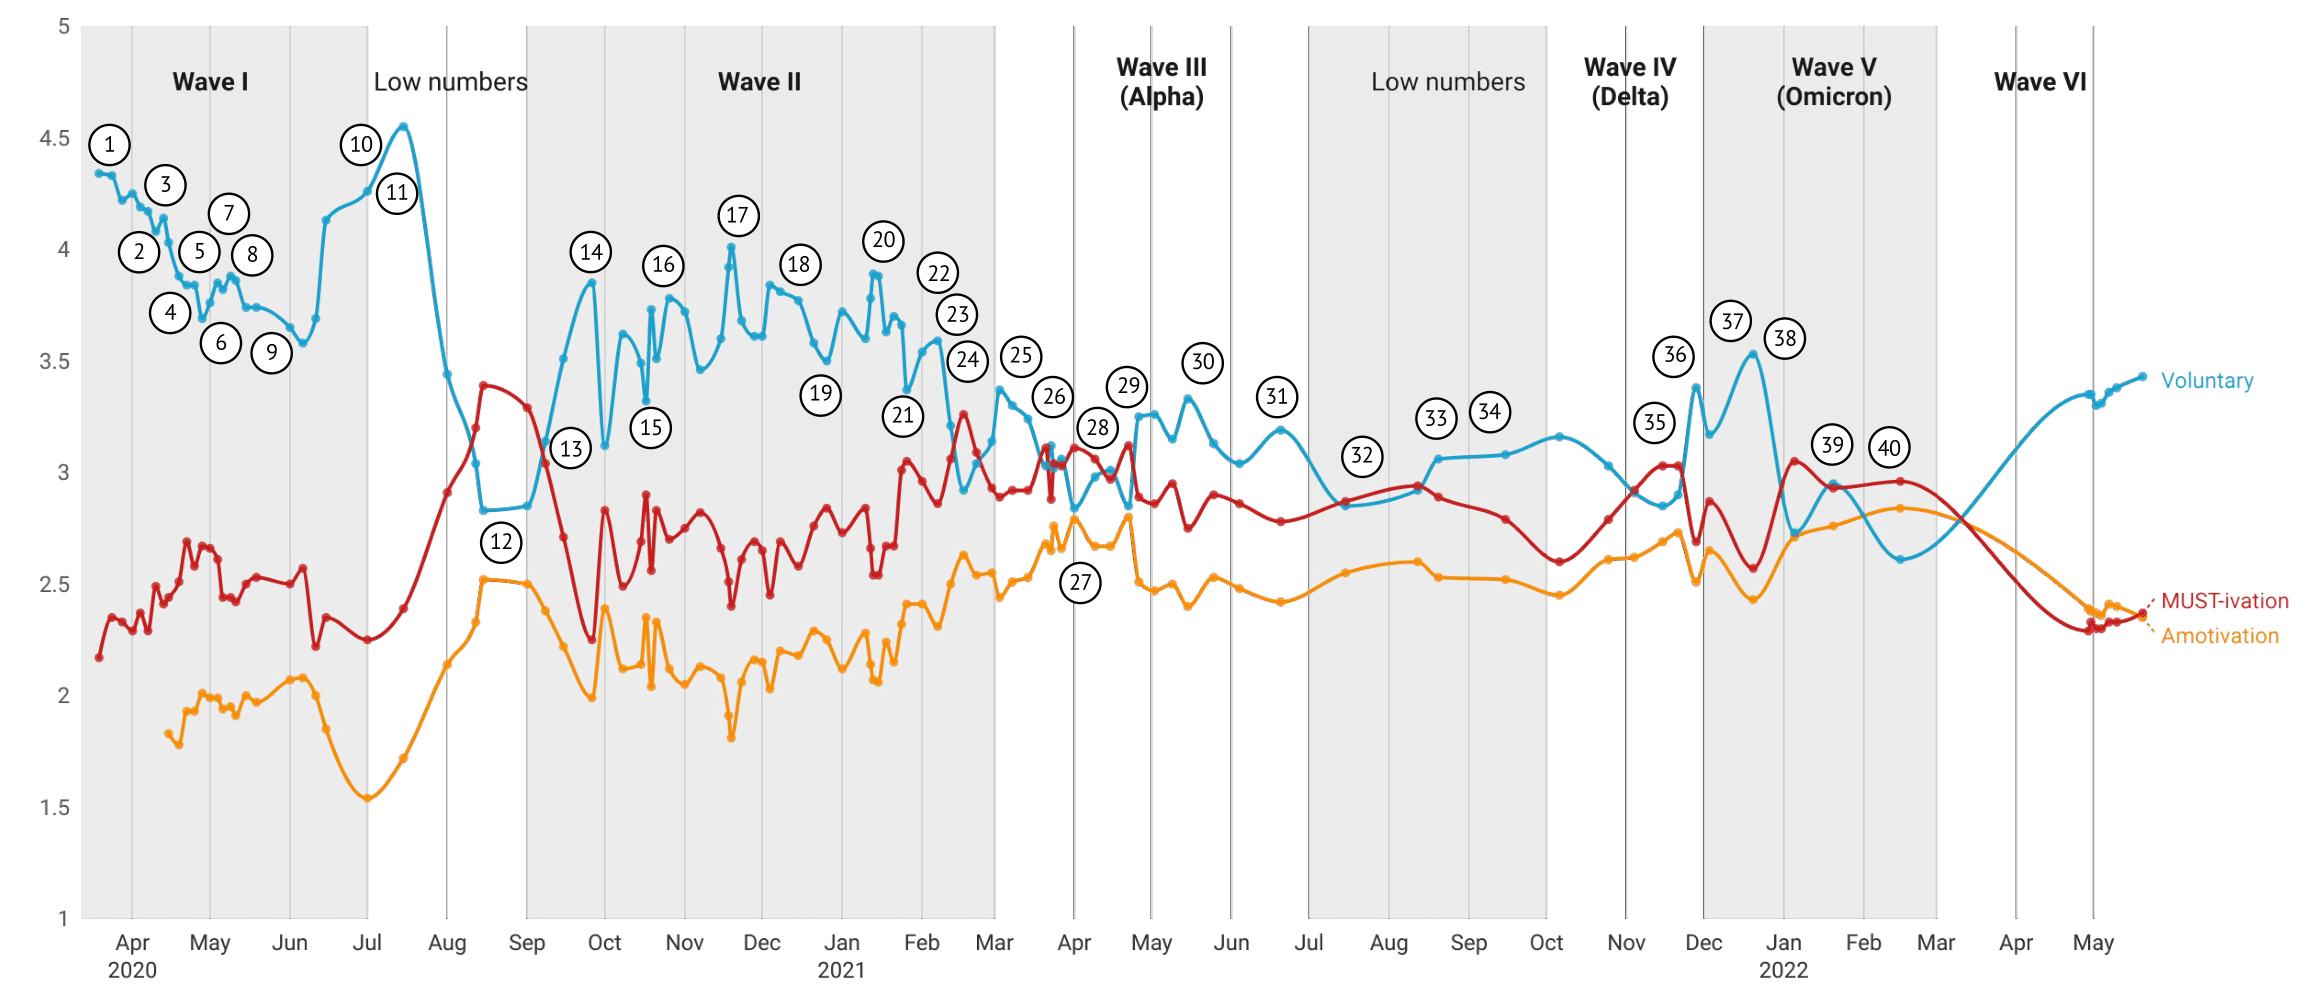
\includegraphics{figures_reports-1.png}

\hypertarget{section-7}{%
\paragraph{2022}\label{section-7}}

\begin{enumerate}
\def\labelenumi{\arabic{enumi}.}
\setcounter{enumi}{39}
\tightlist
\item
  Motivation Barometer (1 February 2022). \textbf{The CST, vaccination
  obligation, 1G policy, or everything on the rocks?} (Report No.~40).
  Ghent, Leuven, Louvain, Bruxelles, Belgium.

  \begin{enumerate}
  \def\labelenumii{\arabic{enumii}.}
  \setcounter{enumii}{38}
  \tightlist
  \item
    Motivation Barometer (19 January 2022). \textbf{Motivation,
    well-being and vaccination attitudes in Omikron times} (Report
    No.~39). Ghent, Leuven, Louvain, Bruxelles, Belgium.
    www.motivationbarometer.com
  \end{enumerate}
\end{enumerate}

\hypertarget{section-8}{%
\paragraph{2021}\label{section-8}}

\begin{enumerate}
\def\labelenumi{\arabic{enumi}.}
\setcounter{enumi}{37}
\tightlist
\item
  Motivation Barometer (21 December 2021). \textbf{Omicron, childhood
  vaccination and end-of-year celebrations: what do we think?} (Report
  No.~38). Ghent, Leuven, Louvain, Bruxelles, Belgium.
  www.motivationbarometer.com

  \begin{enumerate}
  \def\labelenumii{\arabic{enumii}.}
  \setcounter{enumii}{36}
  \tightlist
  \item
    Motivation Barometer (8 December 2021). \textbf{There is still
    support for the measures, but no longer for the corona policy}
    (Report No.~37). Ghent \& Louvain, Belgium.~

    \begin{enumerate}
    \def\labelenumiii{\arabic{enumiii}.}
    \setcounter{enumiii}{35}
    \tightlist
    \item
      Motivation Barometer (16 November 2021). \textbf{On the eve of
      stricter measures: Attitudes toward the new measures and the
      vaccine pass} (Report No.~36). Ghent \& Louvain, Belgium.~

      \begin{enumerate}
      \def\labelenumiv{\arabic{enumiv}.}
      \setcounter{enumiv}{34}
      \tightlist
      \item
        Motivation Barometer (12 November 2021). \textbf{How risk-aware
        and motivated is the population anymore and what is the role of
        the corona pass in this?} (Report No.~35). Ghent \& Louvain,
        Belgium.~

        \begin{enumerate}
        \def\labelenumv{\arabic{enumv}.}
        \tightlist
        \item
          Motivation Barometer (September 9, 2021). \textbf{Is there
          still motivational support for the measures in various
          regions?} (Report No.~34). Ghent \& Louvain, Belgium.~

          \begin{enumerate}
          \def\labelenumvi{\arabic{enumvi}.}
          \tightlist
          \item
            Motivation Barometer (August 17, 2021). \textbf{Update on
            vaccination, motivation and mental health during a
            transition phase.} (Report No.~33). Ghent \& Louvain,
            Belgium.~

            \begin{enumerate}
            \def\labelenumvii{\arabic{enumvii}.}
            \tightlist
            \item
              Motivation Barometer (July 14, 2021). \textbf{Obliging
              health professionals to be vaccinated: a good idea?}
              (Report No.~32). Ghent \& Louvain, Belgium.~

              \begin{enumerate}
              \def\labelenumviii{\arabic{enumviii}.}
              \tightlist
              \item
                Motivation Barometer (June 23, 2021). \textbf{Seduce,
                persuade and/or inform? How to deal with vaccine
                doubters?} (Report No.~31). Ghent \& Louvain, Belgium.~

                \begin{enumerate}
                \def\labelenumix{\arabic{enumix}.}
                \tightlist
                \item
                  Motivation Barometer (May 10, 2021). \textbf{Update on
                  vaccination, motivation, and mental health during a
                  transitional phase} (Report No.~30). Ghent \& Louvain,
                  Belgium.~

                  \begin{enumerate}
                  \def\labelenumx{\arabic{enumx}.}
                  \tightlist
                  \item
                    Motivation Barometer (April 20, 2021). \textbf{Does
                    the prospect of feedbacks motivate the population?}
                    (Report No.~29). Ghent \& Louvain, Belgium.~

                    \begin{enumerate}
                    \def\labelenumxi{\arabic{enumxi}.}
                    \tightlist
                    \item
                      Motivation Barometer (April 6, 2021).
                      \textbf{Vaccination: preferences become clear!}
                      (Report No.~28). Ghent \& Louvain, Belgium.~

                      \begin{enumerate}
                      \def\labelenumxii{\arabic{enumxii}.}
                      \tightlist
                      \item
                        Motivation Barometer (April 1, 2021).
                        \textbf{Saliva testing in schools: impact on
                        mental health, motivation and behavior} (Report
                        No.~27). Ghent \& Louvain, Belgium.~

                        \begin{enumerate}
                        \def\labelenumxiii{\arabic{enumxiii}.}
                        \tightlist
                        \item
                          Motivation Barometer (March 24, 2021).
                          \textbf{Is there motivational willingness for
                          stricter measures?} (Report No.~26). Ghent \&
                          Louvain, Belgium.~

                          \begin{enumerate}
                          \def\labelenumxiv{\arabic{enumxiv}.}
                          \tightlist
                          \item
                            Motivation Barometer (March 2, 2021).
                            \textbf{The corona numbers: motivation
                            matters!} (Report No.~25). Ghent \& Louvain,
                            Belgium.~

                            \begin{enumerate}
                            \def\labelenumxv{\arabic{enumxv}.}
                            \tightlist
                            \item
                              Motivation Barometer (February 14, 2021).
                              \textbf{How can we reinvigorate
                              motivation?} (Report No.~24). Ghent,
                              Belgium.~

                              \begin{enumerate}
                              \def\labelenumxvi{\arabic{enumxvi}.}
                              \tightlist
                              \item
                                Motivation Barometer (February 11,
                                2021). \textbf{(Re)building trust:
                                vaccination and the actors of the
                                pandemic} (Report No.~23). Ghent,
                                Belgium.~

                                \begin{enumerate}
                                \def\labelenumxvii{\arabic{enumxvii}.}
                                \tightlist
                                \item
                                  Motivation Barometer (February 5,
                                  2021). \textbf{Movement as a source of
                                  well-being} (Report No.~22). Ghent,
                                  Belgium.~

                                  \begin{enumerate}
                                  \def\labelenumxviii{\arabic{enumxviii}.}
                                  \tightlist
                                  \item
                                    Motivation Barometer (January 29,
                                    2021). \textbf{At our limits end and
                                    yet persevering} (Report No.~21).
                                    Ghent, Belgium.~

                                    \begin{enumerate}
                                    \def\labelenumxix{\arabic{enumxix}.}
                                    \tightlist
                                    \item
                                      Motivation Barometer (January 15,
                                      2021). \textbf{What are the
                                      psychological conditions to
                                      vaccination?} (Report No.~20).
                                      Ghent, Belgium.~
                                    \end{enumerate}
                                  \end{enumerate}
                                \end{enumerate}
                              \end{enumerate}
                            \end{enumerate}
                          \end{enumerate}
                        \end{enumerate}
                      \end{enumerate}
                    \end{enumerate}
                  \end{enumerate}
                \end{enumerate}
              \end{enumerate}
            \end{enumerate}
          \end{enumerate}
        \end{enumerate}
      \end{enumerate}
    \end{enumerate}
  \end{enumerate}
\end{enumerate}

\hypertarget{section-9}{%
\paragraph{2020}\label{section-9}}

\begin{enumerate}
\def\labelenumi{\arabic{enumi}.}
\setcounter{enumi}{18}
\tightlist
\item
  Motivation Barometer (December 23, 2020). \textbf{Christmas 2020}
  (Report No.~19). Ghent, Belgium.~

  \begin{enumerate}
  \def\labelenumii{\arabic{enumii}.}
  \setcounter{enumii}{17}
  \tightlist
  \item
    Motivation Barometer (December 14, 2020). \textbf{Vaccination
    willingness and motivation} (Report No.~18). Ghent, Belgium.~

    \begin{enumerate}
    \def\labelenumiii{\arabic{enumiii}.}
    \setcounter{enumiii}{16}
    \tightlist
    \item
      Motivation Barometer (23 November 2020). \textbf{What makes for a
      happy Christmas in 2020?} (Report No.~17). Gent, Belgium.~

      \begin{enumerate}
      \def\labelenumiv{\arabic{enumiv}.}
      \setcounter{enumiv}{15}
      \tightlist
      \item
        Motivation Barometer (October 27, 2020). \textbf{Taking a closer
        look at some assumptions about behavior and motivation} (Report
        No.~16). Ghent, Belgium.~

        \begin{enumerate}
        \def\labelenumv{\arabic{enumv}.}
        \tightlist
        \item
          Motivation Barometer (October 14, 2020). \textbf{Even hard
          nuts can be cracked in a motivational way!} (Report No.~15).
          Ghent, Belgium.~

          \begin{enumerate}
          \def\labelenumvi{\arabic{enumvi}.}
          \tightlist
          \item
            Motivation Barometer (September 30, 2020). \textbf{What do
            citizens think of coronabadges and the -barometer? A closer
            look at some motivational tools} (Report No.~14). Ghent,
            Belgium.~

            \begin{enumerate}
            \def\labelenumvii{\arabic{enumvii}.}
            \tightlist
            \item
              Motivation Barometer (September 17, 2020). \textbf{What do
              people think are meaningful alternatives to the current
              bubble concept? The psychological effects of flex bubbles
              and a social carte blanche compared} (Report No.~13).
              Ghent, Belgium.~

              \begin{enumerate}
              \def\labelenumviii{\arabic{enumviii}.}
              \tightlist
              \item
                Motivation Barometer (August 19, 2020). \textbf{The
                population is no longer motivated. How can we create a
                motivational framework} (Report No.~12). Ghent,
                Belgium.~

                \begin{enumerate}
                \def\labelenumix{\arabic{enumix}.}
                \tightlist
                \item
                  Motivation Barometer (July 16, 2020). \textbf{How to
                  maintain high motivation for tracking during this
                  summertime? The role of risk perception, fear, and
                  obligation} (Report No.~11). Ghent, Belgium.~

                  \begin{enumerate}
                  \def\labelenumx{\arabic{enumx}.}
                  \tightlist
                  \item
                    Motivation Barometer (July 1, 2020). \textbf{What
                    makes for an invigorating and rewarding summer
                    vacation in corona times?} (Report No.~10). Ghent,
                    Belgium.~

                    \begin{enumerate}
                    \def\labelenumxi{\arabic{enumxi}.}
                    \tightlist
                    \item
                      Motivation Barometer (May 19, 2020).
                      \textbf{Discomforts of face masks: how we wear
                      them with a smile by encouraging voluntary
                      responsibility} (Report No.~9). Ghent, Belgium.~

                      \begin{enumerate}
                      \def\labelenumxii{\arabic{enumxii}.}
                      \tightlist
                      \item
                        Motivation Barometer (May 14, 2020).
                        \textbf{Student years are the time of your life!
                        Even during corona?} (Report No.~8). Ghent,
                        Belgium.~

                        \begin{enumerate}
                        \def\labelenumxiii{\arabic{enumxiii}.}
                        \tightlist
                        \item
                          Motivation Barometer (May 12, 2020).
                          \textbf{Does `bubbling' on Mother's Day boost
                          our connectedness and motivation?} (Report
                          No.~7). Ghent, Belgium.~

                          \begin{enumerate}
                          \def\labelenumxiv{\arabic{enumxiv}.}
                          \tightlist
                          \item
                            Motivation Barometer (May 5, 2020).
                            \textbf{Motivation rises slightly.
                            Government continue the positive momentum of
                            motivational communication!} (Report No.~6).
                            Ghent, Belgium.~

                            \begin{enumerate}
                            \def\labelenumxv{\arabic{enumxv}.}
                            \tightlist
                            \item
                              Motivation Barometer (April 26, 2020).
                              \textbf{Fatigue during the collective
                              marathon strikes. Evolutions in
                              motivation, mental health and
                              (de)motivating government communication}
                              (Report No.~5). Ghent, Belgium.~

                              \begin{enumerate}
                              \def\labelenumxvi{\arabic{enumxvi}.}
                              \tightlist
                              \item
                                Motivation Barometer (April 21, 2020).
                                \textbf{Motivational willingness for the
                                public marathon is dwindling: the
                                leadership compass as a guide to
                                motivational communication} (Report
                                No.~4). Ghent, Belgium.~

                                \begin{enumerate}
                                \def\labelenumxvii{\arabic{enumxvii}.}
                                \tightlist
                                \item
                                  Motivation Barometer (April 14, 2020).
                                  \textbf{Psychological vitamins in
                                  times of corona fatigue} (Report
                                  No.~3). Ghent, Belgium.~

                                  \begin{enumerate}
                                  \def\labelenumxviii{\arabic{enumxviii}.}
                                  \tightlist
                                  \item
                                    Motivation Barometer (April 8,
                                    2020). \textbf{Is our motivation to
                                    adhere to the measures flattening?
                                    The importance of clear and logical
                                    communication} (Report No.~2).
                                    Ghent, Belgium.~

                                    \begin{enumerate}
                                    \def\labelenumxix{\arabic{enumxix}.}
                                    \tightlist
                                    \item
                                      Motivation Barometer (March 30,
                                      2020). \textbf{How long will we
                                      hold on to these measures? Our
                                      motivation is strong at the
                                      moment!} (Report No.~1). Ghent,
                                      Belgium.~
                                    \end{enumerate}
                                  \end{enumerate}
                                \end{enumerate}
                              \end{enumerate}
                            \end{enumerate}
                          \end{enumerate}
                        \end{enumerate}
                      \end{enumerate}
                    \end{enumerate}
                  \end{enumerate}
                \end{enumerate}
              \end{enumerate}
            \end{enumerate}
          \end{enumerate}
        \end{enumerate}
      \end{enumerate}
    \end{enumerate}
  \end{enumerate}
\end{enumerate}

\hypertarget{conferences}{%
\subsection{Conferences}\label{conferences}}

\hypertarget{section-10}{%
\paragraph{2023}\label{section-10}}

\begin{enumerate}
\def\labelenumi{\arabic{enumi}.}
\setcounter{enumi}{10}
\tightlist
\item
  Waterschoot, J., \& Morbée, S. (2023, September). \textbf{Results of
  the Klimaatmonitor.} Report presented at the Psychology and Society
  Research Day, Brussels, Belgium.

  \begin{enumerate}
  \def\labelenumii{\arabic{enumii}.}
  \setcounter{enumii}{9}
  \tightlist
  \item
    Waterschoot, J. (2023, May-June). \textbf{Motivational Challenges
    during the COVID-19 pandemic: Refreshing Insights from SDT-grounded
    Studies Conducted Across the Globe.} Invited symposium organized at
    the 8th international conference on Self-Determination Theory, 3rd
    Orlando, USA.
  \end{enumerate}
\end{enumerate}

\hypertarget{section-11}{%
\paragraph{2022}\label{section-11}}

\begin{enumerate}
\def\labelenumi{\arabic{enumi}.}
\setcounter{enumi}{8}
\tightlist
\item
  Waterschoot, J. (2022, December). \textbf{The Motivation Barometer:
  The role of needs, risk perception and motivation.} Poster presented
  at the Faculty Research Day (2nd place), Ghent, Belgium.

  \begin{enumerate}
  \def\labelenumii{\arabic{enumii}.}
  \setcounter{enumii}{7}
  \tightlist
  \item
    Waterschoot, J. (2022, October). \textbf{The resilient function of
    the basic psychological needs.} Paper presented at Two-Day Mini
    Conference, Faculty of Psychology and Educational Science, Ghent,
    Belgium.
  \end{enumerate}
\end{enumerate}

\hypertarget{section-12}{%
\paragraph{2019}\label{section-12}}

\begin{enumerate}
\def\labelenumi{\arabic{enumi}.}
\setcounter{enumi}{6}
\tightlist
\item
  Waterschoot, J., Vansteenkiste, M., Verscheuren, K., \& Soenens, B.
  (2019, September).** Towards a refined insight in the shifts in
  adolescents' motivational profiles: A longitudinal study.** Paper
  presented at the European Conference of Developmental Psychology,
  Athene, Greece.

  \begin{enumerate}
  \def\labelenumii{\arabic{enumii}.}
  \setcounter{enumii}{5}
  \tightlist
  \item
    Waterschoot, J., Vansteenkiste, M., Verscheuren, K., \& Soenens, B.
    (2019, August). \textbf{Towards a refined insight in the shifts in
    adolescents' motivational profiles: A longitudinal study.} Paper
    presented at the EARLI conference, Aachen, Germany.

    \begin{enumerate}
    \def\labelenumiii{\arabic{enumiii}.}
    \setcounter{enumiii}{4}
    \tightlist
    \item
      Waterschoot, J., Vansteenkiste, M., \& Soenens, B. (2019, May).
      \textbf{Life ain't no ponyfarm: examining the effectiveness of
      different self-motivating strategies when facing boring
      activities.} Poster presented at the SDT conference, Egmond aan
      Zee, The Netherlands.
    \end{enumerate}
  \end{enumerate}
\end{enumerate}

\hypertarget{section-13}{%
\paragraph{2018}\label{section-13}}

\begin{enumerate}
\def\labelenumi{\arabic{enumi}.}
\setcounter{enumi}{3}
\tightlist
\item
  Waterschoot, J., Soenens, B., \& Vansteenkiste, M. (2018, July).
  \textbf{Effects of Experimentally Induced Choice on Intrinsic
  Motivation in Middle Childhood.} Paper presented at the JURE
  Conference 2018 at the University of Antwerp, Antwerp, Belgium.

  \begin{enumerate}
  \def\labelenumii{\arabic{enumii}.}
  \setcounter{enumii}{2}
  \tightlist
  \item
    Waterschoot, J., Van-der Kaap Deeder, J., \& Vansteenkiste, M.
    (2018, August). \textbf{How do People Handle Competence
    Frustration?: The Role of Resilience and Attentional Bias.} Paper
    presented at the International Conference on Motivation (ICM) at the
    Aarhus University, Aarhus, Denmark.

    \begin{enumerate}
    \def\labelenumiii{\arabic{enumiii}.}
    \setcounter{enumiii}{1}
    \tightlist
    \item
      Waterschoot, J., Soenens, B., \& Vansteenkiste, M. (2018, August).
      \textbf{Effects of Experimentally Induced Choice on Intrinsic
      Motivation in Middle Childhood.} Paper presented at the
      International Conference on Motivation (ICM) at the Aarhus
      University, Denmark.

      \begin{enumerate}
      \def\labelenumiv{\arabic{enumiv}.}
      \tightlist
      \item
        Waterschoot, J., Van-der Kaap Deeder, J., \& Vansteenkiste, M.
        (2018, September). \textbf{The Role of Competence-related
        Attentional Bias and Resilience in Restoring Thwarted Feelings
        of Competence.} Paper presented at the EARA congress at Ghent
        University, Ghent, Belgium
      \end{enumerate}
    \end{enumerate}
  \end{enumerate}
\end{enumerate}

\hypertarget{teaching}{%
\section{\texorpdfstring{Teaching }{Teaching }}\label{teaching}}

\begin{center}\rule{0.5\linewidth}{0.5pt}\end{center}

\hypertarget{experience}{%
\subsection{Experience}\label{experience}}

\emph{2020 - current}

\textbf{Motivation Psychology}: Lecture on Interest Theory and
co-lecturer since 2023 Educational Master

Ghent University Ghent, Belgium.

\emph{2017 - current}

\textbf{Academic Skills}: Supervision, teaching and evaluation of the
courses 2nd Bachelor, Psychology

Ghent University Ghent, Belgium.

\emph{2017 - current}

\textbf{Psychology of the Lifespan}: assigments evaluation of the course
3d Bachelor, Psychology

Ghent University Ghent, Belgium.

\emph{2019 - current}

\textbf{Developmental Psychology}: supervision, organizing, teaching and
evaluating of practical sessions and examination of the course. 1st
Bachelor, Psychology and 2nd Bachelor, Educational Sciences

Ghent University Ghent, Belgium.

\emph{2017 - 2018}

\textbf{Recent Theories on Developmental Psychology}: supervision,
organizing, teaching and evaluating of practical sessions and
examination of the course. 2nd Bachelor, Psychology

Ghent University Ghent, Belgium.

\hypertarget{lectures}{%
\subsection{Lectures}\label{lectures}}

\begin{enumerate}
\def\labelenumi{\arabic{enumi}.}
\setcounter{enumi}{14}
\tightlist
\item
  \textbf{A Brief overview on the Motivation Barometer}, \emph{Science
  meets policy event (14 November 2023)}, Paleis Der Academieën,
  Brussels, Belgium

  \begin{enumerate}
  \def\labelenumii{\arabic{enumii}.}
  \setcounter{enumii}{13}
  \tightlist
  \item
    \textbf{(zelf)motivatie en welzijn bij leerlingen en studenten},
    \emph{GO! Atheneum (5 May 2023)}, Lokeren, Belgium

    \begin{enumerate}
    \def\labelenumiii{\arabic{enumiii}.}
    \setcounter{enumiii}{12}
    \tightlist
    \item
      \textbf{The Impact of the COVID-19 crisis on People's Mental
      Health in Belgium: Insights from the Motivation Barometer} (22
      March, 2023), ``Mental health \& resilience in times of
      polycrisis'', \emph{Superior Health Council (22 March 2023)},
      Brussels, Belgium.
      \url{https://mailchi.mp/health.fgov.be/mental-health-and-resilience-in-times-of-polycrisis\#Form}

      \begin{enumerate}
      \def\labelenumiv{\arabic{enumiv}.}
      \setcounter{enumiv}{11}
      \tightlist
      \item
        \textbf{Werk maken van je motivatie: studenten en docenten} (10
        March 2023), \emph{webbinar}, KU Leuven

        \begin{enumerate}
        \def\labelenumv{\arabic{enumv}.}
        \tightlist
        \item
          \textbf{``Hoe motiveer ik mezelf?'' Motivatie als cruciale
          factor in het gedrag en welbevinden bij (doctoraat)studenten},
          *Uantwerpen, Mind Matters Week (15 November 2022), Antwerp,
          Belgium

          \begin{enumerate}
          \def\labelenumvi{\arabic{enumvi}.}
          \tightlist
          \item
            \textbf{Presentation on Methods, Motivation Barometer,
            Interdisciplinary Symposium}, \emph{KVAB}, Brussels, Belgium

            \begin{enumerate}
            \def\labelenumvii{\arabic{enumvii}.}
            \tightlist
            \item
              \textbf{Presentation on Cluster Analysis} on Research Day
              MOVES (21 December 2021), Ghent, Belgium

              \begin{enumerate}
              \def\labelenumviii{\arabic{enumviii}.}
              \tightlist
              \item
                \textbf{`De Belgische bevolking als leerling in de klas:
                de uitdagingen voor de overheid als leerkracht tijdens
                COVID-19'}, studiedag (21 August 2021),
                \emph{Arteveldehogeschool}, Ghent, Belgium.

                \begin{enumerate}
                \def\labelenumix{\arabic{enumix}.}
                \tightlist
                \item
                  gastcollege \textbf{`de motivatiebarometer'},
                  studiedag, \emph{VIVES hogeschool}, Kortrijk, Belgium

                  \begin{enumerate}
                  \def\labelenumx{\arabic{enumx}.}
                  \tightlist
                  \item
                    \textbf{`De Belgische bevolking als leerling in de
                    klas: de uitdagingen voor de overheid als leerkracht
                    tijdens COVID-19'}, studiedag (10 December 2020),
                    \emph{Arteveldehogeschool}, Ghent, Belgium

                    \begin{enumerate}
                    \def\labelenumxi{\arabic{enumxi}.}
                    \tightlist
                    \item
                      \textbf{`Wanneer de mentale brandstof de motor
                      doet wandelen: presentatie Dodentochtstudie'},
                      open publiek, \emph{Ghent University}, Ghent,
                      Belgium

                      \begin{enumerate}
                      \def\labelenumxii{\arabic{enumxii}.}
                      \tightlist
                      \item
                        \textbf{`Wanneer de mentale brandstof de motor
                        doet wandelen: presentatie Dodentochtstudie op
                        de werkvloer'}, HR groep, Kortrijk, Belgium.

                        \begin{enumerate}
                        \def\labelenumxiii{\arabic{enumxiii}.}
                        \tightlist
                        \item
                          Lecture on `An integrative overview of
                          motivation', ~\emph{The Hult International
                          Business School (15 October 2019)}, London,
                          United Kingdom.

                          \begin{enumerate}
                          \def\labelenumxiv{\arabic{enumxiv}.}
                          \tightlist
                          \item
                            \textbf{`Motivation from a
                            Self-Determination theory perspective'},
                            students, teachers and parents, \emph{Da
                            Vinci Campus (20 March 2018)}, Ronse,
                            Belgium

                            \begin{enumerate}
                            \def\labelenumxv{\arabic{enumxv}.}
                            \tightlist
                            \item
                              \textbf{`A Choice Experiment among
                              elementary school children'}, students
                              Occupational Science,
                              \emph{Arteveldehogeschool (12 March
                              2015)}, Ghent, Belgium
                            \end{enumerate}
                          \end{enumerate}
                        \end{enumerate}
                      \end{enumerate}
                    \end{enumerate}
                  \end{enumerate}
                \end{enumerate}
              \end{enumerate}
            \end{enumerate}
          \end{enumerate}
        \end{enumerate}
      \end{enumerate}
    \end{enumerate}
  \end{enumerate}
\end{enumerate}

\hypertarget{master-theses-supervision}{%
\subsection{Master theses supervision}\label{master-theses-supervision}}

\begin{enumerate}
\def\labelenumi{\arabic{enumi}.}
\setcounter{enumi}{27}
\tightlist
\item
  Roos Mertens (current). \textbf{`Ik (b)en de groep': een longitudinale
  studie naar het effect van collectieve behoeftebevrediging op het
  individu.} Niet-gepubliceerde Master Thesis, Universiteit Gent.
  (Promotor: J. Waterschoot)

  needs

  \begin{enumerate}
  \def\labelenumii{\arabic{enumii}.}
  \setcounter{enumii}{26}
  \tightlist
  \item
    Hanne Van De Keere (current). \textbf{``Hoe kan ik mezelf
    motiveren?'' De ontwikkeling van een interventie in een
    studentenpopulatie.} Niet-gepubliceerde Master Thesis, Universiteit
    Gent. (Promotor: J. Waterschoot)

    zelfmotivatie

    \begin{enumerate}
    \def\labelenumiii{\arabic{enumiii}.}
    \setcounter{enumiii}{25}
    \tightlist
    \item
      Eline Buseyne \& Lise Vanbrabant (current). \textbf{In welke mate
      sluimert de COVID-19 crisis nog door? Een longitudinale studie
      naar de kijk van mensen op huidige maatschappelijke thema's.}
      Niet-gepubliceerde Master Thesis, Universiteit Gent. (Promotor: J.
      Waterschoot)

      covid19

      \begin{enumerate}
      \def\labelenumiv{\arabic{enumiv}.}
      \setcounter{enumiv}{24}
      \tightlist
      \item
        Charlotte Buelens (current). \textbf{Werken strengere
        maatregelen steeds demotiverend? Een vignetten studie naar de
        rol van overheidscommunicatie over het klimaat.}
        Niet-gepubliceerde Master Thesis, Universiteit Gent. (Promotor:
        J. Waterschoot)

        climate change

        \begin{enumerate}
        \def\labelenumv{\arabic{enumv}.}
        \tightlist
        \item
          Marie Vankeirsbilck (current). \textbf{Hoe is de motivatie en
          het psychologisch welzijn bij studenten geëvolueerd tussen
          2020 (pre-corona) en 2022 (post-corona)?} Niet-gepubliceerde
          Master Thesis, Universiteit Gent. (Promotor: M. Vansteenkiste)

          covid19

          \begin{enumerate}
          \def\labelenumvi{\arabic{enumvi}.}
          \tightlist
          \item
            Peeters, Pieter (2023). \textbf{Heeft het begin van de
            coronacrisis geleid tot een verandering in het
            waardenpatroon van mensen?} Niet-gepubliceerde Master
            Thesis, Universiteit Gent. (Promotor: M. Vansteenkiste)

            covid19

            \begin{enumerate}
            \def\labelenumvii{\arabic{enumvii}.}
            \tightlist
            \item
              Van Baelen, Kato (2023). \textbf{Zelfmotivatie voeden
              vanuit de opvoeding.} Niet-gepubliceerde Master Thesis,
              Universiteit Gent. (Promotor: M. Vansteenkiste)

              selfmotivation

              \begin{enumerate}
              \def\labelenumviii{\arabic{enumviii}.}
              \tightlist
              \item
                Verhulst, Sarah (2023). \textbf{Zelfmotivatie voeden
                vanuit de opvoeding.} Niet-gepubliceerde Master Thesis,
                Universiteit Gent. (Promotor: M. Vansteenkiste)

                selfmotivation

                \begin{enumerate}
                \def\labelenumix{\arabic{enumix}.}
                \tightlist
                \item
                  Vanhaverbeke, Alice (2023). \textbf{Longitudinale
                  profielen in middelbare school motivatie.}
                  Niet-gepubliceerde Master Thesis, Universiteit Gent.
                  (Promotor: M. Vansteenkiste)

                  school

                  \begin{enumerate}
                  \def\labelenumx{\arabic{enumx}.}
                  \tightlist
                  \item
                    Helpers, Margot (current). \textbf{Do blue-collar
                    and white-collar workers benefit from the same
                    ABC-recipe and need-supportive leadership? A
                    comparative study of basic psychological needs.}
                    Niet-gepubliceerde Master Thesis, Universiteit Gent.
                    (Promotor: M. Vansteenkiste, Co-promotor: N.
                    Aelterman)

                    work

                    \begin{enumerate}
                    \def\labelenumxi{\arabic{enumxi}.}
                    \tightlist
                    \item
                      Belgrado, Laura (2022). \textbf{De mediërende rol
                      van zelfmotivatie tussen emotieregulatie en
                      verveling.} Niet-gepubliceerde Master Thesis,
                      Universiteit Gent. (Promotor: M. Vansteenkiste)

                      selfmotivation

                      \begin{enumerate}
                      \def\labelenumxii{\arabic{enumxii}.}
                      \tightlist
                      \item
                        Bogaerts, Liesa (2022). \textbf{Zelfmotivatie,
                        tweede lockdown, verveling en kwalitatieve
                        codering.} Niet-gepubliceerde Master Thesis,
                        Universiteit Gent. (Promotor: B. Soenens)

                        selfmotivation

                        \begin{enumerate}
                        \def\labelenumxiii{\arabic{enumxiii}.}
                        \tightlist
                        \item
                          Truyen, Isabel (2021). \textbf{Een
                          microbenadering naar de relatie tussen
                          autonomie-ondersteunend opvoeden en
                          emotieregulatie bij adolescenten.}
                          Niet-gepubliceerde Master Thesis, Universiteit
                          Gent. (Promotor: M. Vansteenkiste) ~

                          parenting

                          \begin{enumerate}
                          \def\labelenumxiv{\arabic{enumxiv}.}
                          \tightlist
                          \item
                            De Quick, Lotte (2021). \textbf{Even
                            stilstaan in het hier en nu: verveling in
                            tijdens van corona. De mediërende rol van
                            zelfmotivatie in de verbanden van
                            afstandsonderwijs en mindfulness met
                            verveling, vitaliteit, geboeidheid door de
                            leerstof in een groep van adolescenten.}
                            Niet-gepubliceerde Master Thesis,
                            Universiteit Gent. (Promotor: M.
                            Vansteenkiste)

                            selfmotivation

                            \begin{enumerate}
                            \def\labelenumxv{\arabic{enumxv}.}
                            \tightlist
                            \item
                              Pede, Sarah (2021). \textbf{De
                              psychologische basisbehoeftes: autonomie,
                              verbondenheid en competentie in tijden van
                              corona. Een kwalitatief-kwantitatieve
                              benadering van het bubbelen op moederdag
                              en de rol van de psychologische
                              achtergrondvariabelen.} Niet-gepubliceerde
                              Master Thesis, Universiteit Gent.
                              (Promotor: M. Vansteenkiste)

                              needs

                              \begin{enumerate}
                              \def\labelenumxvi{\arabic{enumxvi}.}
                              \tightlist
                              \item
                                Bruteyn, Sarah (2021). \textbf{Werkt
                                zelfmotivatie de verveling weg? Een
                                studie naar de rol van zelfmotivatie op
                                verveling en vitaliteit tijdens het werk
                                in tijdens van COVID-19.}
                                Niet-gepubliceerde Master Thesis,
                                Universiteit Gent. (Promotor: M.
                                Vansteenkiste)

                                selfmotivation

                                \begin{enumerate}
                                \def\labelenumxvii{\arabic{enumxvii}.}
                                \tightlist
                                \item
                                  Vanacker, Liesanne (2021).
                                  \textbf{Persoonlijkheid als sleutel
                                  tegen verveling tijdens de lockdown.
                                  Een onderzoek naar de dispositionele
                                  rol van neuroticisme en mindfulness
                                  bij levenstevredenheid en verveling
                                  tijdens de COVID-19 lockdown.}
                                  Niet-gepubliceerde Master Thesis,
                                  Universiteit Gent. (Promotor: M.
                                  Vansteenkiste)

                                  covid19

                                  \begin{enumerate}
                                  \def\labelenumxviii{\arabic{enumxviii}.}
                                  \tightlist
                                  \item
                                    Sercu, Jade (2021). \textbf{Hoe
                                    motiveer ik mijn kind voor een
                                    vervelende taak? De rol van
                                    verschillende ouderlijke strategieën
                                    met een brede opvatting van types
                                    beloning.} Niet-gepubliceerde Master
                                    Thesis, Universiteit Gent.
                                    (Promotor: M. Vansteenkiste)

                                    selfmotivation

                                    \begin{enumerate}
                                    \def\labelenumxix{\arabic{enumxix}.}
                                    \tightlist
                                    \item
                                      Hernandez, Nicaurys (2021).
                                      \textbf{Wegwijs in onze eigen
                                      emoties in tijden van een
                                      pandemie. Een onderzoek naar
                                      zelfmotivatie als mediator in het
                                      verband tussen emotieregulatie en
                                      verveling.} Niet-gepubliceerde
                                      Master Thesis, Universiteit Gent.
                                      (Promotor: M. Vansteenkiste)

                                      covid19

                                      \begin{enumerate}
                                      \def\labelenumxx{\arabic{enumxx}.}
                                      \tightlist
                                      \item
                                        Van Houtte, Camille (2021).
                                        \textbf{Motivatie als brandstof
                                        voor de Dodentocht. Een
                                        mixed-method studie met
                                        kwantitatieve metingen en
                                        kwalitatieve diepte-interviews.}
                                        Niet-gepubliceerde Master
                                        Thesis, Universiteit Gent.
                                        (Promotor: M. Vansteenkiste)

                                        motivation

                                        \begin{enumerate}
                                        \def\labelenumxxi{\arabic{enumxxi}.}
                                        \tightlist
                                        \item
                                          De Lille, Maud (2020).
                                          \textbf{De motivatie achter de
                                          Dodentocht: een heldentocht of
                                          een lijdensweg?}
                                          Niet-gepubliceerde Master
                                          Thesis, Universiteit Gent.
                                          (Promotor: M. Vansteenkiste)

                                          motivation

                                          \begin{enumerate}
                                          \def\labelenumxxii{\arabic{enumxxii}.}
                                          \tightlist
                                          \item
                                            Dewilde, Bjarne (2020).
                                            \textbf{Even stilstaan in
                                            het hier en nu: waarom deze
                                            taak als vervelend aan-
                                            voelt. De rol van
                                            mindfulness in onze
                                            capaciteit tot
                                            zelfmotivatie.}
                                            Niet-gepubliceerde Master
                                            Thesis, Universiteit Gent.
                                            (Promotor: M. Vansteenkiste)

                                            selfmotivation

                                            \begin{enumerate}
                                            \def\labelenumxxiii{\arabic{enumxxiii}.}
                                            \tightlist
                                            \item
                                              Koekelkoren, Juno (2020).
                                              \textbf{Mijn doelen in een
                                              deelname aan de
                                              Dodentocht: een
                                              kwalitatieve analyse.}
                                              Niet-gepubliceerde Master
                                              Thesis, Universiteit Gent.
                                              (Promotor: M.
                                              Vansteenkiste)

                                              motivation

                                              \begin{enumerate}
                                              \def\labelenumxxiv{\arabic{enumxxiv}.}
                                              \tightlist
                                              \item
                                                Wydooghe, Lore (2020).
                                                \textbf{``Hoe motiveer
                                                ik mezelf voor een
                                                vervelende taak?'': een
                                                onderzoek naar de
                                                wortels van
                                                zelf-motivatie.}
                                                Niet-gepubliceerde
                                                Master Thesis,
                                                Universiteit Gent.
                                                (Promotor: M.
                                                Vansteenkiste)

                                                motivation

                                                \begin{enumerate}
                                                \def\labelenumxxv{\arabic{enumxxv}.}
                                                \tightlist
                                                \item
                                                  Zels, Julie (2020).
                                                  \textbf{De motivatie
                                                  achter de Dodentocht:
                                                  een heldentocht of een
                                                  lijdensweg?}
                                                  Niet-gepubliceerde
                                                  Master Thesis,
                                                  Universiteit Gent.
                                                  (Promotor: M.
                                                  Vansteenkiste)~

                                                  motivation

                                                  \begin{enumerate}
                                                  \def\labelenumxxvi{\arabic{enumxxvi}.}
                                                  \tightlist
                                                  \item
                                                    Casteleyn, Demi
                                                    (2020).
                                                    \textbf{``Help, ik
                                                    doe dit écht niet
                                                    graag!'': hoe ouders
                                                    de capaciteit tot
                                                    zelf-motivatie
                                                    kunnen
                                                    versterken.''}
                                                    Niet-gepubliceerde
                                                    Master Thesis,
                                                    Universiteit Gent.
                                                    (Promotor: M.
                                                    Vansteenkiste)

                                                    selfmotivation

                                                    \begin{enumerate}
                                                    \def\labelenumxxvii{\arabic{enumxxvii}.}
                                                    \tightlist
                                                    \item
                                                      Swinnen, Kato
                                                      (2019).
                                                      \textbf{``Smartphonenende''
                                                      ouders: hoe
                                                      beschikbaar zijn
                                                      ze voor hun
                                                      kinderen en hoe
                                                      voeden ze hun
                                                      kinderen op?}
                                                      Niet-gepubliceerde
                                                      Master Thesis,
                                                      Universiteit Gent.
                                                      (Promotor: M.
                                                      Vansteenkiste)

                                                      parenting

                                                      \begin{enumerate}
                                                      \def\labelenumxxviii{\arabic{enumxxviii}.}
                                                      \tightlist
                                                      \item
                                                        Vermeire,
                                                        Ephraïm (2018)
                                                        \textbf{Mag
                                                        plezier bestaan
                                                        in de klas? Een
                                                        differentiatie
                                                        van plezier en
                                                        de samenhang met
                                                        aspecten van
                                                        zelfbeheersing
                                                        in klassikale
                                                        context.}
                                                        Niet-gepubliceerde
                                                        Master Thesis,
                                                        Universiteit
                                                        Gent. (Promotor:
                                                        M.
                                                        Vansteenkiste)

                                                        school
                                                      \end{enumerate}
                                                    \end{enumerate}
                                                  \end{enumerate}
                                                \end{enumerate}
                                              \end{enumerate}
                                            \end{enumerate}
                                          \end{enumerate}
                                        \end{enumerate}
                                      \end{enumerate}
                                    \end{enumerate}
                                  \end{enumerate}
                                \end{enumerate}
                              \end{enumerate}
                            \end{enumerate}
                          \end{enumerate}
                        \end{enumerate}
                      \end{enumerate}
                    \end{enumerate}
                  \end{enumerate}
                \end{enumerate}
              \end{enumerate}
            \end{enumerate}
          \end{enumerate}
        \end{enumerate}
      \end{enumerate}
    \end{enumerate}
  \end{enumerate}
\end{enumerate}

\hypertarget{media-podcasts}{%
\section{\texorpdfstring{Media \& Podcasts
}{Media \& Podcasts }}\label{media-podcasts}}

\begin{center}\rule{0.5\linewidth}{0.5pt}\end{center}

\emph{02/08/2022}

80-plussers zijn al aan vijfde vaccinprik toe

\href{download/press/covid/destand80.pdf}{DS }

\emph{23/06/2022}

Podcast `Motivationbarometer', episode: Risk perception

\href{https://open.spotify.com/episode/2GjCmZTxjONfmgYBNhPNJu?si=7d5da8bf43104ce5}{Spotify
}

\emph{06/05/2021}

Ruim zeven op de tien studenten willen vaccin

\href{download/press/covid/20210506Ruim-zeven-op-de-tien-studenten-willen-vaccin.pdf}{DM
}

\emph{18/06/2020}

``Al zevenduizend wandelaars voor 100 km Covid Challenge''

\href{download/press/covid/20200618zevenduizend-wandelaars-voor-100-km-Covid-Cha.pdf}{Nieuwsblad
}

\emph{20/05/2020}

De quarantaineparadox: hoe corona ons tijdsbesef verandert

\href{download/press/covid/20200520knack.pdf}{Knack }

\emph{28/04/2020}

Coronavirus - Psychologen: ``motivatiecampagne is cruciaal om deze
volksmarathon vol te houden''

\href{download/press/covid/20200428volksmarathon-vol-t.pdf}{Belga }

\emph{06/03/2020}

Universiteit Gent doet onderzoek naar deelname aan de Dodentocht

\href{download/press/dodentocht/download-clip_20200306_gazet-van-antwerpen-mechelen-waas_p-22-23.pdf}{GVA
}
\href{download/press/dodentocht/20200306_Het-Laatste-Nieuws_p-0_Dodentocht-Goesting-zorgt-voor-betere-motivatie-dan-druk.pdf}{HLN
(1) }
\href{download/press/dodentocht/download-clip_20200307_het-laatste-nieuws-mechelen-lier_p-40-41.pdf}{HLN
(2) } \href{download/press/dodentocht/vrt_be.pdf}{VRT }
\href{download/press/dodentocht/rtv_be.pdf}{RTV }
\href{download/press/dodentocht/Radio1_06032020.mp4}{Radio 1 }
\href{download/press/dodentocht/Radio2_Antwerpen_06032020.aac}{Radio 2
Antw } \href{download/press/dodentocht/Radio2_OVL_06032020.aac}{Radio 2
O-Vl } \href{download/press/dodentocht/JoeFM_06032020.aac}{Joe FM }

\hypertarget{awards}{%
\section{\texorpdfstring{Awards }{Awards }}\label{awards}}

\begin{center}\rule{0.5\linewidth}{0.5pt}\end{center}

\textbf{October 21, 2021}

The `Royal Flemish Academy of Belgium' (KVAB) and the `Young Academy'
annually hand out the \textbf{`Distinctions for Scientific
Communication'} to scientists with an exceptional merit in scientific
communication. The Year Prizes are awarded to researchers who have
devoted themselves intensively over the past two years to a concrete
project in the field of science communication.

Text on the website: \emph{Maarten Vansteenkiste, Joachim Waterschoot
and Sofie Morbée are awarded the Annual Scientific Communication Prize
for their communication on the motivation barometer in the context of
the coronapandemic. The motivation barometer has gradually developed
into an important policy instrument. There is also strong appreciation
for the accompanying excellent website on which the findings are
disseminated to a very wide audience through dozens of accessible
reports, opinion pieces and media interventions, and which provides an
insight into the scientific process.}

\href{https://www.youtube.com/watch?v=Q_h7re70y_U\&feature=emb_title}{Watch\ldots{}
}
\href{https://kvab.be/nl/prijzen/jaarprijzen-wetenschapscommunicatie}{Read
more\ldots{}}


\includegraphics{unnamed.png}

\hypertarget{research-visit}{%
\section{\texorpdfstring{Research visit
}{Research visit }}\label{research-visit}}

\begin{center}\rule{0.5\linewidth}{0.5pt}\end{center}


\includegraphics{ntnu_hoeyde_eng.png} \textbf{Invited research visit}
\emph{November 18 - 24, 2022}

NTNY, Trondheim, Norway Invitation from Prof.~Dr.~Jolene Van der
Kaap-Deeder to teach and to support the research group in data analysis
of different research projects, doing this in R.
\href{https://kvab.be/nl/prijzen/jaarprijzen-wetenschapscommunicatie}{Link
to research group}

\hypertarget{extracurricular-activities}{%
\section{Extracurricular activities}\label{extracurricular-activities}}

\begin{center}\rule{0.5\linewidth}{0.5pt}\end{center}

\textbf{2023}

\begin{itemize}
\tightlist
\item
  Organization of \textbf{scientific day} for +300 attendees with
  international speakers like Ryan, Mageau, etc. (`Strengthening young
  people's resilience together: The motivational role of teachers,
  parents and caregivers', website:
  \url{https://www.studiedag-veerkracht.be/}). July 7, 2023, Faculty of
  Psychology and Educational Science, Ghent, Belgium.
\end{itemize}

\textbf{2021 -- current}

\begin{itemize}
\tightlist
\item
  \textbf{Alumni functioning}: GAP (member of steering group: secretary
  and co-director since 2023)\\
\item
  \textbf{Representative for pre- and post-docs}: Department meeting,
  Faculty Board, Commission of Scientific Research
\end{itemize}

\textbf{2019-- current}

\begin{itemize}
\tightlist
\item
  Organization of \textbf{IPSAS} meetings on department (Informal
  Presentations for Starters And Seniors): once each 6 months (from 2019
  on) with invited speakers and workshops (e.g., scientific poster
  construction).
\end{itemize}

\textbf{2017-- current}

\begin{itemize}
\tightlist
\item
  \textbf{Alumni functioning}: GAP (member of steering group:
  secretary)\\
\item
  \textbf{Representative for pre- and post-docs}: Department meeting
\end{itemize}

\textbf{2015 -- 2017}

\begin{itemize}
\tightlist
\item
  \textbf{Alumni functioning}: GAP (voluntarily member)\\
\item
  \textbf{Student council} of the Faculty of Psychology and Educational
  Sciences (PPSR): President, Member of GSR (General Student
  Representation), Commission of Reception, Commission of Finance and
  Staff, Commission of Scientific Research, Faculty Board, Commission of
  the Course of Education Psychology
\end{itemize}

\end{document}
